\section{Supersimetría}
\label{cap:susy}

Una de las teorías de física más allá del SM más motivadas desde el punto de
vista teórico es la Supersimetría, ya que resuelve algunos de los problemas
fundamentales del mismo. Entre otras cosas provee una solución al problema de
jerarquía, como así también una derivación del mecanismo de Higgs, permite la
unificación de las fuerzas del SM y hasta provee una conexión entre estas y la
gravedad, además de proporcionar un candidato para la materia oscura.

%% Sin embargo el concepto de Supersimetría no nació por estos motivos. Durante el
%% a\~no 1966 Hironari Miyazawa propuso la existencia de una supersimetría que
%% relacionaba mesones y bariones en el contexto de la física hadrónica, aunque
%% este trabajo fue ignorado en ese momento.
%% Durante 1971 y 1972 varios físicos redescubrieron la supersimetría de manera
%% independiente en el contexto de la teoría cuántica de campos, una nueva simetría
%% del espacio-tiempo y los campos fundamentales que establecía una relación entre
%% las partículas elementales con naturaleza cuántica distinta (bosones y
%% fermiones), y unificaba el espacio-tiempo con las simetrías internas de los
%% fenómenos microscópicos. Este redescubrimiento apareció ligado a las primeras
%% teorías de cuerdas.
%% Finalmente, Julius Wess y Bruno Zumino (en 1974) identificaron el carácter
%% renormalizable de la teorías de campos supersimétricas en cuatro dimensiones, y
%% luego Abdus Salam y sus estudiantes introdujeron las primeras aplicaciones para
%% física de partículas. La primera versión realista de un SM supersimétrico fue
%% propuesta durante 1977 por Pierre Fayet y se conoce como MSSM.

En esta sección se introduce el concepto de Supersimetría y se detallan algunas
características fenomenológicas que resultan importantes para esta Tesis.


\subsection{Problema de jerarquía}

El {\SM} de la física de altas energías descripto en el capítulo anterior, con
el agregado de la masa de los neutrinos, y el descubrimiento del bosón de Higgs,
ha tenido un gran éxito en la descripción de los fenómenos conocidos hasta la
escala del {\tev} explorados por los experimentos en los últimos a\~nos.
%% A pesar de esto, resulta claro que el Modelo Est\'andar no es una teoria definitiva y va a tener que
%% ser extendida para describir la f\'isica de altas energ\'ias.
A pesar de esto, no hay dudas respecto a que será necesaria una nueva teoría
a la escala reducida de Planck $M_P = (8\pi G_\text{Newton})^{-1/2} = 2.4 \times
10^{18} \gev$ , donde los efectos cuánticos gravitacionales son importantes.
Se sabe que tiene que existir nueva física en los 16 órdenes de magnitud en
energía entre el territorio explorado cerca de la escala electrodébil y la
escala de Planck. El sólo hecho de que la relación $M_P/M_W$ es tan grande es
una gran pista para la física más allá del {\SM}, por el llamado \emph{problema
  de jerarquía}. Este no es una dificultad intrínseca del SM, sino una
preocupante sensibilidad del potencial de Higgs a nueva física en casi cualquier
extensión imaginable del SM.

La parte eléctricamente neutra del campo de Higgs del SM es un escalar complejo
$H$ con un potencial clásico $V=m_H^2 |H|^2 + \lambda|H|^4$. El SM necesita un
valor de expectación del vacío (VEV) para $H$ en el mínimo del potencial no
nulo. Esto ocurre si $\lambda>0$ y $m_H^2<0$, resultando en $\avg{H} =
\sqrt{-m_H^2/2\lambda}$. Como experimentalmente sabemos que $\avg{H}$ es
aproximadamente 174 \gev, de las medidas de las propiedades de las interacciones
débiles, el valor de $m_H^2$ debe ser del orden de $-(100 \gev)^2$.

\begin{figure}[!htbp]
  \centering \begin{tikzpicture}[node distance=1cm and 1 cm]

  \coordinate[vertex, label=above:$H$] (v1);
  \coordinate[vertex, right=of v1] (v2);
  \coordinate[vertex, right=of v2] (v3);
  \coordinate[vertex, right=of v3] (v4);

  \draw[higgs] (v1) -- (v2);
  \draw[higgs] (v3) -- (v4);

  \draw[fermion] (1.5, 0) circle (0.5);
  \node at (1.5, 0.75) {$f$};

\end{tikzpicture}

  \caption{Correcciones cuánticas a un loop al parámetro de masa del Higgs
    $m_H^2$ debido a la masa de un fermión de Dirac $f$.}
  \label{fig:higgs_correction_f}
\end{figure}

El problema es que $m_H^2$ recibe grandes correcciones cuánticas de los efectos
virtuales de cada partícula que se acopla, directa o indirectamente, el
campo de Higgs. Por ejemplo, en la \cref{fig:higgs_correction_f} tenemos una
corrección a $m_H^2$ del loop que contiene un fermión de Dirac $f$ con masa
$m_f$. Si el campo de Higgs se acopla a $f$ con un término en el lagrangiano
igual a $-\lambda_f H \bar{f}f$, el diagrama de Feynman en la
\cref{fig:higgs_correction_f} genera una corrección:

\begin{equation}
  \Delta m_H^2 = -\frac{|\lambda_f|^2}{8\pi^2} \Lambda^2_{\text{UV}} %+ \ldots
  \label{eq:higgs_corr_f}
\end{equation}
%
donde $\Lambda_\text{UV}$ es el corte usado para regular la integral en el
\emph{loop}. Debe ser interpretado como la m\'inima escala de energ\'ia a la
cual entra la nueva física para alterar el comportamiento de la teoría a altas
energías. Los puntos suspensivos representan términos proporcionales a $m_f^2$,
que crecen a lo sumo logaritmicamente con $\Lambda_\text{UV}$. Cualquiera de los
leptones o quarks del SM puede jugar el rol de $f$ (para el caso de quarks la
correcciónón tiene que ser multiplicada por 3 para tener en cuenta el color) y
la correción m\'as grande va a ser cuando $f$ es el quark \emph{top} con
$\lambda_f \approx 1$.

El problema aparece si $\Lambda_\text{UV}$ es del orden de $M_P$, ya que la
corrección a $m_H^2$ es 30 órdenes de magnitud más grande que el valor requerido
de $m_H^2 \sim (100 \gev)^2$. Este es sólo un problema para las correcciones al
cuadrado de la masa del bosón de Higgs escalar, porque las correcciones
cuánticas a las masas de los fermiones y los bosones de gauge no tienen una
sensibilidad cuadrática directa a $\Lambda_\text{UV}$ como la que están en la
\cref{eq:higgs_corr_f}. Sin embargo, los quarks, leptones y los bosones de gauge
electrodébiles $Z^0$, $W^{\pm}$ del SM, todos obtienen masa de $\avg{H}$, por
lo tanto el espectro completo de masas del SM es directa o indirectamente
sensible a la escala de corte $\Lambda_\text{UV}$.

Se puede pensar que la solución es elegir un $\Lambda$ no demasiado grande, pero
igualmente se debería mezclar todavía algo de nueva física a la escala
$\Lambda_\text{UV}$ que no solo altere los propagadores en el \emph{loop}, sino que
corte la integral. Esto no es fácil en una teoría cuyo lagrangiano no contiene
mas de dos derivadas, y las teorías de mayor orden en derivadas generalmente
sufren de fallas de unitariedad o causalidad.
%In string theories, loop integrals are nevertheless cut off at high Euclidean
%% momentum p by factors e −p /Λ UV . However, then Λ UV is a string scale that
%% is usually † thought to be
%% not very far below M P . Furthermore, there are contributions similar to eq.
%% (1.2) from the virtual effects
%% of any arbitrarily heavy particles that might exist, and these involve the
%% masses of the heavy particles,
%% not just the cutoff.

\begin{figure}[!htbp]
  \centering \begin{tikzpicture}[node distance=1cm and 1 cm]

  \coordinate[vertex, label=above:$H$] (v1);
  \coordinate[vertex, right=of v1] (v2);
  \coordinate[vertex, right=of v2] (v3);
  \coordinate[vertex, right=of v3] (v4);

  \draw[higgs] (v1) -- (v2);
  \draw[higgs] (v2) -- (v3);
  \draw[higgs] (v3) -- (v4);

  \draw[higgs] (1.5, 0.5) circle (0.5);

  \node at (1.5, 1.25) {$S$};

\end{tikzpicture}

  \caption{Correcciones cuánticas a un loop al parametro de masa del Higgs
    $m_H^2$ debido a la masa de un campo escalar $S$.}
  \label{fig:higgs_correction_s}
\end{figure}

En el caso de que exista un escalar complejo pesado $S$ con masa $m_S$ que se
acopla al Higgs con un término en el Lagrangiano $-\lambda_S \abs{H}^2
\abs{S}^2$, el diagrama de Feynman es el que se muestra en la
\cref{fig:higgs_correction_s} y este da lugar a una corrección:

\begin{equation}
  \Delta m_H^2 = \frac{\lambda_S^2}{16\pi^2} \left[ \Lambda^2_\text{UV} - 2
    m_S^2 \ln (\Lambda^2_\text{UV}/m_S) + \ldots \right]
  \label{eq:higgs_corr_s}
\end{equation}

%% Puede ser que el boson de Higgs no sea una fundamenta, como en modelos technicolor, o modelos en
%% los cuales el Higgs es compuesto.
Si el bosón de Higgs es una partícula fundamental y hay física a una escala
mucho mayor que la escala electrodébil, existen dos opciones: hacer
alguna suposición bizarra de que no existe ninguna partícula de mayor masa o
efectos que se acoplen (incluso indirectamente o extremadamente débiles) con el
campo escalar de Higgs, o es necesario algún tipo de cancelación entre las
distintas contribuciones a $\Delta m_H^2$.

%------
% SUSY
%------
\subsection{Supersimetría}

La cancelación sistemática de las contribuciones a $\Delta m_H^2$ puede ser
realizada por una simetría. Comparando las
\cref{eq:higgs_corr_f,eq:higgs_corr_s} se puede ver que existe una diferencia
de signo
entre las contribuciones del \emph{loop} fermiónico y bosónico. La cancelación de todas
estas contribuciones a las masas escalares no solo es posible, sino que es
inevitable, si se considera la existencia de una simetría que relacione fermiones y
bosones. A esta simetría se la denomina supersimetría o SUSY.

Una transformación supersimétrica convierte un estado bosónico en uno
fermiónico, y viceversa. El operador $Q$ que genera estas transformaciones debe
ser un espinor anticonmutativo, con

\begin{equation}
  Q \ket{\text{bosón}} = \ket{\text{fermión}}, \quad \quad Q
  \ket{\text{fermión}} = \ket{\text{bosón}}
\end{equation}

Los espinores son intrínsecamente objetos complejos, por lo tanto el conjugado
hermitico de $Q$ es también un generador de la simetría. Debido a que $Q$ y
$Q^\dagger$ son operadores fermiónicos, llevan momento angular de espín $\frac{1}{2}$, por
lo tanto es claro que SUSY debe ser una simetría espacio-temporal y los
operadores $Q$ y $Q^\dagger$ deben satisfacer un álgebra de la siguiente forma,

\begin{align}
  \{Q, Q^\dagger\} &= P^\mu \\
  \{Q, Q\} &= \{Q^\dagger, Q^\dagger\} = 0 \\
  [P^\mu, Q] &= [P^\mu, Q^\dagger] = 0
\end{align}
%
donde $P^\mu$ es el momento generador de las traslaciones
espacio-temporales.

Los estados de partícula de una teoría supersimétrica son representados en el
álgebra de SUSY como supermultipletes. Cada supermultiplete contiene
ambos estados, fermión y bosón, que son comúnmente llamados supercompa\~neros
uno de otro.

Los generadores $Q$ y $Q^\dagger$ conmutan con los generadores de las
transformaciones de gauge, por lo tanto las partículas en un mismo
supermultiplete tienen que estar en la misma representación del grupo de gauge,
y tener la misma carga eléctrica, isospin y color. Y como el operador de masa
$-P^2$ también conmuta con los generadores y con todos los operadores de
rotación y traslación, deberán tener los mismos autovalores de $-P^2$, y
entonces la misma masa.

Es fácil probar que cada supermultiplete tiene que contener igual número de
grados de libertad fermiónico que bosónico, $n_B = n_F$. La posibilidad más
simple para satisfacer esto es tener un único fermión de Weyl ($n_F=2$) y dos
escalares reales (cada uno con $n_B=1$). Estos dos escalares se suelen poner
como un único campo escalar complejo. Esta combinación de un fermión de Weyl de
dos componentes y un campo escalar complejo es llamado un supermultiplete
quiral (ó escalar).

Otra posibilidad es que el supermultiplete contenga un bosón vectorial de espín
1. Para que la teoría sea renormalizable, tiene que ser un bosón de gauge no
masivo, al menos antes de que la simetría de gauge sea espontáneamente rota. En
este caso, este bosón contiene dos estados de helicidad, $n_B=2$. Por lo tanto
su supercompa\~nero es un fermión de Weyl de espín $\frac{1}{2}$, con dos estados de
helicidad, $n_F=2$. Si en vez de esto, se intenta usar un fermión de espín $\frac{3}{2}$
la teoría no sería renormalizable. Los bosones de gauge deben transformar como
la representación adjunta del grupo de gauge, por lo que sus compañeros
fermiónicos, llamados \emph{gauginos}, también. Esta combinación de gauginos
de espín $\frac{1}{2}$ y bosones de gauge de espín 1 es llamada supermultiplete de
gauge (ó vectorial).

Si se incluye la gravedad, el gravitón de espín 2 (con dos estados de helicidad,
$n_B=2$) tiene un supercompañero de espín $\frac{3}{2}$ llamado \emph{gravitino}.

Existen otras combinaciones posibles de partículas que pueden satisfacer estas
condiciones, pero siempre se reducen a combinaciones de supermultipletes
quirales o de gauge, excepto en ciertas teorías con supersimetría extendida.
Estas teorías tienen más de una copia de los generadores $Q$ y $Q^\dagger$, pero no
son muy prometedoras desde el punto de vista fenomenológico. La teoría no
extendida y fenomenológicamente viable es llamada generalmente $N=1$, donde $N$
se refiere al número de supersimetrías (el número de las distintas copias de
$Q$ y $Q^\dagger$).


%------
% MSSM
%------
\subsection{Modelo Mínimo Estándar Supersimétrico}

En una extensión supersimétrica del SM, cada una de las partículas fundamentales
conocidas esta contenida en un supermultiplete quiral o de gauge, y debe tener
un supercompa\~nero con espín que difiere en $\frac{1}{2}$ de este. La extensión que
requiere la introducción de la mínima cantidad de partículas se conoce como
\emph{Modelo Mínimo Estándar Supersimétrico}, o MSSM.

%% The first step in understanding the exciting phenomenological consequences of
%% this prediction is to decide exactly how the known particles fit into supermultiplets, and to give them
%% appropriate names.

Sólo los supermultipletes quirales pueden contener fermiones cuya parte
izquierda y derecha transforman de forma diferente bajo el grupo de gauge. Todos
los fermiones del SM (quarks y leptones) tienen esta propiedad, por lo tanto
deben ser miembros de supermultipletes quirales. Los nombres de los compañeros
de espín 0 de los quarks o leptones son construidos anteponiendo una ``s'' (de
\emph{scalar}), y son llamados \emph{squarks} y \emph{sleptones}, o
\emph{sfermiones}. La parte izquierda y derecha de los quarks y leptones son
fermiones de Weyl con diferentes propiedades de transformación de gauge del SM,
entonces cada uno debe tener un compañero escalar complejo. Por ejemplo, los
supercompañeros de la parte izquierda y derecha del campo de Dirac de los
electrones son llamadas {\selL} y {\selR}, aunque el subíndice no se refiere a
la helicidad de los slectrones (ya que tiene espín 0) sino a la de sus supercompañeros.
Lo mismo ocurre para {\smuL}, {\smuR}, {\stauL} y {\stauR}. Los neutrinos del SM
son siempre izquierdos por lo que sus supercompañeros se denotan {\snu}. Y
para los quarks se tiene {\squarkL} y {\squarkR}, con $q = u, d, s, c, b, t$. Las
interacciones de gauge de cada uno de los campos de squarks y sleptones son las
mismas que la de los correspondientes fermiones del SM.

El bosón escalar de Higgs debe estar en un supermultiplete quiral ya que tiene
espín 0. Dada la naturaleza de los campos quirales introducidos en la
implementación de SUSY, el campo escalar de Higgs no es suficiente para dar masa
a los fermiones de helicidad izquierda y derecha. Se debe agregar un nuevo campo
escalar para compensar. En el SM, el campo de Higgs es un doblete, y de los
cuatro grados de libertad solo uno permanece como consecuencia del rompimiento
de la simetría electrodébil, resultando en un bosón de Higgs. Los dos dobletes
de Higgs del MSSM son:

\begin{equation}
  H_u = \binom{H_u^+}{H_u^0}, \quad \quad \quad H_d = \binom{H_d^0}{H_d^-}
\end{equation}

Los bosones vectoriales del SM tienen que estar en supermultipletes de gauge.
Sus supercompañeros fermiónicos son llamados \emph{gauginos}. Las interacciones
de gauge de color $\text{SU}(3)_C$ de QCD son mediadas por el gluón, cuyo
compañero supersimétrico de espín $\frac{1}{2}$ es el \emph{gluino}. La simetría
electrodébil $\text{SU}(2)_L \times \text{U}(1)_Y$ esta asociada con los bosones
de espín 1, $W^+, W^0, W^-$ y $B^0$, cuyos compañeros de espín $\frac{1}{2}$ son $\susy{W}^+,
\susy{W}^0, \susy{W}^-$ y $\susy{B}^0$, y son llamados \emph{winos} y
\emph{bino}. Después de la ruptura de la simetría electrodébil, los auto-estados
$W^0$ y $B^0$ se mezclan para dar $Z^0$ y $\gamma$.

En la \cref{tab:sparticles} se puede ver las distintas partículas que
conforman el MSSM.


\begin{table}[ht!]
  \centering
  \begin{tabular}{x{4cm} x{4cm} x{4cm}}
    \hline
    {\bf Supermultiplete} & {\bf Bosón} & {\bf Fermión} \\ %& SU(3), SU(2), U(1) \\
    \hline
    gluon, gluino & $g$ & \gluino \\ %& 8, 1, 0 \\
    \hline
    W, wino & $W^\pm$, $W^0$  & $\winopm, \winozero$ \\ %& 1, 3, 0 \\

    B, bino &   $B$ & \bino \\ %& 1, 1, 0 \\
    \hline
    slepton, lepton & $(\snu, \susy{e})_L$ & $(\nu, e)_L$ \\%& 1, 2, -1/2 \\
    ($\times 3$ generaciones)     & $e_\mathrm{R}$ & $e_\mathrm{R}$ \\ %& 1, 1, -2 \\

    \hline

    squark, quark & $(\susy{u}_\mathrm{L}, \susy{d}_\mathrm{L})$ & $(u_\mathrm{L}, d_\mathrm{L})$ \\ %& 3, 2, 1/6 \\
    ($\times 3$ generaciones)  & $\susy{u}_\mathrm{R}$ & $u_\mathrm{R}$ \\ %& 3, 1, -2/3 \\
                  & $\susy{d}_\mathrm{R}$ & $d_\mathrm{R}$ \\ %& 3, 1, 1/3 \\

    \hline

    Higgs, higgsinos & $(H_d^0, H_d^-)$ & $(\susy{H}_d^0, \susy{H}_d^-)$ \\ %& 1, 2, -1/2 \\
                     & $(H_u^+, H_u^0)$ & $(\susy{H}_u^+, \susy{H}_u^0)$ \\ %& 1, 2, 1/2 \\

    \hline

  \end{tabular}
  \caption{Supermultipletes quirales y de gauge del MSSM.}
  \label{tab:sparticles}
\end{table}



\subsubsection{Espacio de parámetros del MSSM}

Los parámetros del MSSM se pueden describir considerando de forma separada el
sector que conserva SUSY del sector de rompimiento de SUSY
\cite{PDG,Haber:1993wf}. Primero se tienen los parámetros usuales del SM: los
acoplamientos de gauge $g_s$, $g$ y $g'$, correspondientes al grupo de gauge
SU(3), SU(2) y U(1), respectivamente. Las constantes de acoplamiento entre
fermiones y Higgs: $\lambda_u$, $\lambda_d$ y $\lambda_e$. % (correspondientes
al acoplamiento de una generación).
%de quarks y leptones izquierdos y derechos, y sus super-compa\~neros,
%a los bosones y Higgs y higgsinos).
Otro parámetro es el parámetro de masa del supercampo de Higgs $\mu$.

Los demás parámetros del MSSM aparecen de los términos de rompimiento soft de
SUSY. Estos incluyen tres parámetros de masa de los gauginos ($M_3, M_2$ y
$M_1$), cinco parámetros de masa escalares para squarks y sleptones
$M^2_{\susy{Q}}$, $M^2_{\susy{U}}$, $M^2_{\susy{D}}$, $M^2_{\susy{L}}$ y
$M^2_{\susy{E}}$, términos de interacción triliniares Higgs-squark-squark y
Higgs-slepton-slepton ($A_t$, $A_b$ y $A_\tau$), y los parámetros de masa del
sector de Higgs ($m^2_{1H}$, $m^2_{2H}$ y $m^2_{12}$). Luego del rompimiento de
la simetría electrodébil, los parámetros $m^2_{1H}$, $m^2_{2H}$ y $m^2_{12}$
pueden ser expresados en términos de dos valores de expectación del vacío ($v_1$
y $v_2$) y una masa física de Higgs (en general se elige la masa del Higgs
escalar CP-impar, $m_{A^0}$). Como $v_1^2+v_2^2=(246 \gev)^2$ esta fijo por la
masa del $W$ o $Z$, se suele escribir en términos de un parámetro definido como
el cociente $\tan \beta \equiv v_2/v_1$.

En un modelo con una sola generación de quarks, leptones y sus
supercompa\~neros, la lista anterior tiene 14 nuevos parámetros. En el modelo
completo de tres generaciones, el número de nuevos parámetros es sustancialmente
mayor ya que los parámetros de masa de los squarks y sleptones y los parámetros
$A$ serán matrices de $3 \times 3$, y la posibilidad de mezcla entre
generaciones puede llevar a complicaciones adicionales. Sin embargo, no todos
estos parámetros son físicos. Algunos de estos parámetros pueden ser eliminados
expresando los autoestados de interacción en términos de los autoestados de
masa, con la apropiada redefinición de los campos del MSSM para remover los
grados de libertad no físicos. El análisis de la referencia
\cite{Dimopoulos:1995ju} muestra que el MSSM posee 124 parámetros
independientes. De estos, 18 corresponden a los parámetros del SM, uno
corresponde al sector de Higgs (el análogo a la masa del Higgs del SM), y 105
son nuevos parámetros del modelo.

Realizar predicciones y análisis fenomenológicos con esta cantidad de parámetros
es impracticable, por lo cual es necesario realizar suposiciones para reducir
los grados de libertad. Es debido a este motivo que no existe una definición
precisa del MSSM y es importante conocer cuales son las suposiciones que se han
hecho cuando se estudia un determinado análisis.

En un tratamiento fenomenológico completo todos los parámetros del MSSM deberían
dejarse libres y determinarse a partir de los datos observados. Luego de que los
parámetros hayan sido medidos, se podría intentar extraer información de la física
subyacente que esta asociada con escalas de energía mayores a la de los
experimentos.
%%\note{Agregar límites a los parametros?}

%% Ya que la conjetura principal de SUSY esta motivada por el
%% intento de embed la física de bajas energías en un modelo más fundamental, es
%% apropiado explotar esta motivación en contraining los parámetros de SUSY a
%% bajas energías.


\subsubsection{Paridad R}

La forma general del superpotencial del MSSM tiene como inconveniente que el
número leptónico y bariónico no es una cantidad conservada. Esto implica que el
protón puede decaer a través del intercambio del compañero escalar del quark
$d$. Esto se contradice claramente con la evidencia experimental, que establece
un límite superior en la vida media del protón que es $> 10^{30}$ a\~nos a $90\%$ CL\cite{PDG}.

Para evitar este problema, la estrategia más comúnmente utilizada es introducir
una nueva simetría. Esta simetría se la conoce como paridad-R y puede escribirse
como,

\begin{equation}
  P_R = (-1)^{3(B-L)+ 2s}
\end{equation}
%
donde $B$ y $L$ son respectivamente el número bariónico y leptónico, y $s$ es el
espín de la partícula. Las partículas supersimétricas tienen $P_R = -1$, mientras
que las partículas del SM tienen $P_R = +1$.

Si la paridad-R es exactamente conservada, no puede haber mezcla entre las
spartículas y las partículas del SM. Cada vértice de interacción en la teoría
contiene entonces un número par de spartículas, lo cual conlleva a tres
consecuencias fenomenológicas de extrema importancia:

\begin{itemize}
\item En experimentos de colisionadores, las partículas supersimétricas pueden
  sólo ser producidas en número par, en general de a dos.
\item La partícula supersimétrica más liviana, llamada LSP, es estable y no tiene
  ninguna partícula con $P_R = -1$ a la cual decaer. Si
  la LSP es eléctricamente neutra, interactúa solo de forma débil con la materia
  ordinaria, y por lo tanto resulta en un candidato muy atractivo para la
  materia oscura no bariónica que es requerida por la cosmología. Desde el punto de
  vista experimental la LSP solo será visible a través de la energía faltante
  dejada en el detector.
\item Cada partícula supersimétrica que no sea la LSP debe decaer eventualmente
  en un estado que contenga un número impar de LSP (en general una).
\end{itemize}



\subsubsection{El espectro de masas del MSSM}

Una característica importante del MSSM es que las nuevas partículas, que están
listadas en la \cref{tab:sparticles}, no son necesariamente autoestados de masa
de la teoría. Después del rompimiento de la simetría electrodébil
y de la supersimetría, puede haber mezcla entre los gauginos y higgsinos, y
entre los squarks y sleptones y los Higgs escalares que tienen la misma carga
eléctrica. La única excepción es el gluino.

En el MSSM, la descripción del rompimiento de la simetría electrodébil es un
poco más complicada que en el SM debido al hecho de que hay dos dobletes
complejos de Higgs $H_u$ y $H_d$ en vez de solo uno.
Examinar los distintos autovalores de masa de la teoría, no es un análisis
trivial, ya que cualquier conjunto de partículas con los mismos números
cuánticos puede mezclarse. En las siguientes secciones se analizan los distintos
sectores del modelo.

%% \note{Explicar mínimamente el rompimiento}

%% En el MSSM los higgsinos neutros y los gauginos se mezclan para
%% formar los cuatro neutralinos:
%% \ninoone, \ninotwo, \ninothree\ y \ninofour.
%% Y de forma similar los higgsinos cargados y los winos dan lugar
%% a los dos charginos, \chinoonepm\ y \chinotwopm.

%% con un total de 8 grados de libertad, 3 de los cuales se pierden en
%% el rompimiento
%% de la simetria EW. Por lo tanto quedan 5 bosones de Higgs en el MSSM:
%% $h^0, H^0, H^+, H^-, A^0$.
%% El más liviano de los 5 es $h^0$, el cual es el más similar al del SM.

%% We have now assembled all the pieces of the MSSM.
%% To proceed, we next examine
%% the mass eigenstates of the theory. This is not a completely trivial analysis, since
%% any set of particles of a given spin, B, L and SU(3)C × U(1)EM quantum numbers
%% can mix.


\begin{itemize}\itemsep0.2cm\parskip0.2cm

\item Sector de Higgs

Los campos escalares de Higgs en el MSSM consisten en dos dobletes de
$\text{SU}(2)_\text{L}$ complejos $H_u$ y $H_d$, con 8 grados de libertad
escalares. Después del rompimiento de la simetría electrodébil, tres de estos
son bosones de Nambu-Goldstone, que se convierten en los modos longitudinales de
los bosones vectoriales $Z$ y $W^\pm$. Los restantes cinco grados de libertad
producen los cinco bosones de Higgs físicos del modelo: el par de bosones de
Higgs cargados $H^\pm$; un bosón de Higgs neutral CP-impar $A^0$; y los bosones
de Higgs neutral CP-par, $H^0,h^0$, donde por convención $h^0$ es más liviano
que $H^0$.


\item Neutralinos y Charginos %%}\label{sec:mass_NC}

Los higgsinos y los gauginos electrodébiles se mezclan entre ellos debido al
efecto del rompimiento de la simetría electrodébil. Los higgsinos neutros
($\susy{H}_u^0$ y $\susy{H}_d^0$) y los gauginos neutros (\bino, \winozero) se
combinan para formar cuatro autoestados de masa llamados \emph{neutralinos}.
Los higgsinos cargados ($\susy{H}_u^+$ y $\susy{H}_d^-$) y los winos (\winop y
\winom) se mezclan para formar dos autoestados de masa con carga $\pm 1$
llamados \emph{charginos}.

La mezcla de los gauginos y higgsinos cargados está descripta a orden árbol por la matriz de $2\times 2$:

\begin{equation}
  M_{C} = \left(
  \begin{array}{cc}
    \M{2} & \frac{1}{\sqrt{2}} g v_u \\
    \frac{1}{\sqrt{2}} g v_d & \mu \\
  \end{array}
  \right)
\end{equation}
%
la cual se debe diagonalizar para determinar los estados físicos y las masas de los charginos.
Estos dos autoestados de masa se indican con {\chinoonepm} y
{\chinotwopm} y su masa esta dada por:

\begin{equation}
  M^2_{\susy{\chi}_{1,2}} = \frac{1}{2} \left\{ M^2 + \mu^2 + 2 m_W^2 \mp
  [(M^2-\mu^2)^2 + 4 m_W^4 \cos^2 2\beta + 4 m_W^2 (M^2+\mu^2 + 2 M \mu \sin
    2\beta)]^{1/2} \right\}
\end{equation}

%% En la base de autoestados de gauge $\psi^0 = (\bino, \winozero, \susy{H_d^0}, \susy{H}_u^0)$,
%% la parte de masa del neutralino del Lagrangiano es

%% \begin{equation}
%%   \mathcal{L}_\text{neutralino mass} = -\frac{1}{2} (\psi^0)^T M_{\nino} \psi^0 + c.c.
%% \end{equation}
%% %
%% donde

En el caso de los neutralinos la matriz de masa es:

\begin{equation}
  M_{N} = \left(
  \begin{array}{cccc}
    \M{1} & 0 & -c_\beta s_W m_Z & s_\beta s_W m_Z \\
    0 & \M{2} & c_\beta c_W m_Z & -s_\beta c_W m_Z \\
    -c_\beta s_W m_Z & c_\beta c_W m_Z & 0 & -\mu \\
    s_\beta s_W m_Z & s_\beta -c_W m_Z & -\mu & 0 \\
  \end{array}
  \right)
\end{equation}

Para el caso de los neutralinos se utiliza la siguiente notación $\tilde{\chi}^0_{i}$ ($i=1,2,3,4$)
y al igual que en el caso de los charginos son ordenados de forma ascendente según su masa (es decir,
el $i=1$ es el más liviano).

%% El neutralino más liviano
%% {\ninoone}, suele ser la LSP, salvo que exista un {\gravino} más liviano
%% o que la paridad-R no se conserve.

%% Los autoestados de masas y la matriz de mezcla $N_{ij}$ pueden obtenerse en termino de los parámetros
%% \M{1}, \M{2}, $\mu$ y $\tan\beta$.

%% El sector de los neutralinos esta determinado por tres parámetros reales, \M{1}, $\tan\beta$ y
%% $\mu$ (como también por supuesto $m_Z$ y $\theta_W$).

Si un estado de chargino o neutralino se aproxima a un estado particular de
gaugino o higgsino, es conveniente usar la nomenclatura correspondiente. Si
$M_1$ y $M_2$ son pequeñas comparadas a $m_Z$ y $|\mu|$, el neutralino más
liviano va a ser puramente fotino. Si $M_1$ y $m_Z$ son pequeños comparados a
$M_2$ y $|\mu|$, entonces el neutralino más liviano va a ser puramente bino. Si
$M_2$ y $m_Z$ son pequeñas comparadas con $M_1$ y $|\mu|$, el par de charginos
más liviano y neutralino va a constituir un triplete de winos puro degenerado en
masas. Finalmente, si $|\mu|$ y $m_Z$ son chicos comparados con $M_1$ y $M_2$,
el neutralino más liviano va a ser un higgsino puro. Cada unos de los casos
anteriores va a llevar a un fenomenología muy distinta.


\item Gluino

Como el gluino es un fermión de color con ocho componentes, no puede mezclarse con ninguna
otra partícula del MSSM (aunque haya violación de paridad-R). El parámetro de
masa del gluino $M_3$ esta relacionado con los parámetros de masa de bino y wino
($M_1$ y $M_2$) por la siguiente aproximación:

\begin{equation}
  M_3 : M_2 : M_1 \quad \sim \quad 6 : 2 : 1
\end{equation}
%
valida cerca de la escala del {\tev} (suponiendo que tienen un valor de masa común
en la escala GUT). Por este motivo es razonable considerar que el gluino es
considerablemente más pesado que los neutralinos y charginos.


\item Squarks y sleptones

Cualquier par de escalares con la misma carga eléctrica, paridad-R y color
pueden mezclarse entre ellos. Después del agregado de los términos del
rompimiento soft de la supersimetría, los auto-estados de masa de los squarks y
sleptones del MSSM pueden obtenerse diagonalizando tres matrices de $6\times6$
para squarks up, down y sleptones cargados, y una matriz adicional de $3\times
3$ para los sneutrinos. La primera y segunda familia de squarks y sleptones
terminan con siete pares casi degenerados. En contraste, la tercera familia de
squarks y sleptones pueden tener masas muy distintas y una mezcla importante de
a pares $(\stopL, \stopR)$, $(\sbottomL, \sbottomR)$ y $(\stauL, \stauR)$.

Para un cierto fermión $f$ de la tercera generación, las matrices hermiticas en
la base de los auto-estados de gauge $(\sfermionL, \sfermionR)$ pueden ser
diagonalizadas por una matriz unitaria para dar los auto-estados de masa
denotados por $(\sfermionone, \sfermiontwo)$:

\begin{equation}
  m_{\widetilde{f}_{\mathrm{1,2}}}^2 = m^2_f + \frac{1}{2} \left[
    m_{\sfermionL}^2 + m_{\sfermionR}^2 \mp \sqrt{(m_{\sfermionL}^2 -
      m_{\sfermionR}^2)^2 + 4 m_f^2 C^2} \right]
\end{equation}
%
con $m_{\sfermionone}^2 < m_{\sfermiontwo}^2$, donde el parámetro $C$ es un
valor conocido que puede ser obtenido de los acoplamientos Yukava y soft y el
cociente de los VEVs de los $H_u^0$ y $H_d^0$. Dado que la masa del top $m_t$ es
muy alta, la mezcla es particularmente importante para el sector del $\stop$.
Esto genera una gran diferencia entre las masas de los dos auto-estados de los
stops, dejando posiblemente un stop mucho más liviano a los demás squarks.

\end{itemize}


\subsubsection{Decaimiento de spartículas}

\begin{itemize}\itemsep0.2cm\parskip0.2cm

\item Neutralinos y charginos

Como cada neutralino y chargino contiene al menos una mezcla de los gauginos
electrodébiles {\bino}, $\tilde W^0$ o $\susy{W}^{\pm}$ , heredan los
acoplamientos de intensidad electrodébil a los pares de fermiones escalares. Si
los sleptones o squarks son lo suficientemente livianos, un neutralino o
chargino va a decaer a un par leptón+slepton o quark+squark. También pueden
decaer en un neutralino o chargino más liviano y un Higgs escalar o un bosón
de gauge electrodébil. Los posibles decaimientos son

\begin{align*}
  &\susy{N}_i \to Z \susy{N}_j, \quad W \susy{C}_j, \quad h^0 \susy{N}_j, \quad
  \ell \susy{\ell}, \quad \nu \susy{\nu}, \quad [A^0 \susy{N}_j, \quad H^0
    \susy{N}_j, \quad H^{\pm} \susy{C}_j^{\mp}, \quad q \susy{q}],
  \\ &\susy{C}_i \to W \susy{N}_j, \quad Z \susy{C}_1, \quad h^0 \susy{C}_1,
  \quad \ell \susy{\nu}, \quad \nu \susy{\ell}, \quad [A^0 \susy{C}_1, \quad H^0
    \susy{C}_1, \quad H^{\pm} \susy{N}_j, \quad q \susy{q}']
\end{align*}
%
donde los estados finales entre corchetes son los cinemáticamente menos
probables.


\item Sleptones

Los sleptones puede decaer en un lepton y un chargino o neutralino,

\begin{align}
  \slepton &\to \ell \nino, \nu\chinopm \\ \snu &\to \nu\nino, \ell\chinopm
\end{align}

Como los sleptones derechos no se acoplan al gaugino de $\text{SU}(2)_\text{L}$,
comúnmente prefieren el decaimiento directo a $\ell\ninoone$.


\item Gluino

El gluino solo puede decaer a través de un squark, ya sea on-shell o virtual. Si
el decaimiento a dos cuerpos está abierto, este va a dominar debido al
acoplamiento gluino-quark-squark tiene intensidad QCD. En el caso de que todos
los squarks sean más pesados que el gluino, este va a decaer sólo vía squarks
virtuales.

\begin{align}
  &\gluino \to q\susy{q}, \\
  &\gluino \to qq\nino, qq^\prime \chinopm
\end{align}


\item Squarks

Los squarks puede tener decaimiento a dos cuerpos en un squark-gluino si es
cinematicamente permitido, porque tiene acoplamiento QCD. Por otro
lado, los squarks pueden decaer en un quark y un neutralino/chargino.

\begin{equation}
  \susy{q} \to q\gluino, \, q\nino, \, q^\prime \chinopm
\end{equation}

%% El gluino, chargino o neutralino que resulta del decaimiento de un squark
%% va a decaer
%% The gluino, chargino or neutralino resulting from the squark decay will in turn
%% decay, and so on, until a final state containing χ  ̃ 1 is reached. This results in
%% numerous and complicated decay chain possibilities called cascade decays.

\end{itemize}

%---------------------
% Rompimiento de SUSY
%---------------------
\subsection{Rompimiento de la Supersimetría}

Los supermultipletes quirales y de gauge de la \cref{tab:sparticles} conforman
el contenido de partículas del MSSM. Desde el punto de vista experimental,
ninguna de las compa\~neras supersimétricas de las partículas del SM han sido
observadas hasta el momento. Si la supersimetría no estuviera rota, deberían
existir selectrones con una masa igual a $m_e \sim 0.511 \mev$, y lo mismo para
los demás sleptones y squarks. Y también deberían existir los gluinos y fotinos
sin masa. El hecho de que no hayan sido descubiertas hasta el momento es motivo
evidente de que SUSY es una simetría que esta rota en el estado de vacío elegido
por la naturaleza.

Pero una de las principales motivaciones para introducir esta nueva simetría fue
que las divergencias cuadráticas en el cuadrado de las masas escalares podían
anularse a todo orden en teoría de perturbaciones, y eso está garantizado solo
si esta simetría no esta rota. Para que SUSY todavía pueda proveer la solución
al problema de jerarquía incluso en presencia del rompimiento de esta, las
relaciones entre los acoplamientos adimensionales que están en la teoría antes
del rompimiento deben mantenerse. Para que esto suceda, el rompimiento de la
supersimetría debe ser \emph{soft}, es decir, el Lagrangiano efectivo del MSSM
tiene que poder ser escrito como:

\begin{equation}
  \mathcal{L} = \mathcal{L}_\text{SUSY} + \mathcal{L}_\text{soft}
\end{equation}
%
donde $\mathcal{L}_\text{SUSY}$ contiene todas las interacciones de gauge y de
Yukawa y preserva la invarianza supersimétricas, y $\mathcal{L}_\text{soft}$
viola supersimetría pero contiene solo términos de masa y parámetros de
acoplamientos con dimensión de masa positiva. Si la escala de masa más grande
asociada con los términos soft se llama $m_\text{soft}$, las correcciones
adicionales no supersimétricas al cuadrado de la masa escalar del Higgs debe
anularse en el límite $m_\text{soft} \to 0$.

Debido a que la diferencia de masas entre las partículas conocidas del SM y sus
súper-compañeras son determinadas por los parámetros $m_\text{soft}$ que
aparecen en $\mathcal{L}_\text{soft}$, las masas de las partículas
supersimétricas no pueden ser demasiado grandes. De otra forma perderíamos la
solución al problema de jerarquía.

Por otro lado, también existe una razón por la cual las partículas
supersimétricas deben ser lo suficientemente pesadas para no haber sido
descubiertas hasta ahora. Todas las demás partículas del MSSM que han sido
observadas tienen algo en común: deberían no tener masa en ausencia del
rompimiento de la simetría electrodébil. En particular, las masas de los
bosones $W^\pm$, $Z^0$ y todos los quarks y leptones son iguales al producto de
constantes de acoplamiento adimensionales por el $\avg{H} \sim 174 \gev$,
mientras que el fotón y el gluon necesitan ser no masivos por la invarianza de
gauge electromagnética y de QCD. Por el contrario, todas las partículas del MSSM
no descubiertas tienen la propiedad contraria. Cada una de ellas pueden tener un
término de masa en el Lagrangiano en ausencia del rompimiento de la simetría
electrodébil.

En el MSSM, el rompimiento de SUSY es introducido explícitamente. El rompimiento
de una simetría global siempre implica un modo no masivo de Nambu-Goldstone con
los mismos números cuánticos que el generador de la simetría rota. En el caso de
la supersimetría global, el generador es la carga fermionica $Q_\alpha$, por lo
tanto la partícula de Nambu-Goldstone tiene que ser un fermión de Weyl no masivo
neutro, llamado \emph{goldstino}. Es claro ahora que el rompimiento espontáneo
de la supersimetría requiere la extensión del MSSM. El rompimiento espontáneo de
SUSY tiene que ocurrir en un \emph{sector oculto} de partículas que no tienen
acoplamientos directos con los supermultipletes quirales (\emph{sector visible})
del MSSM. Sin embargo, estos dos sectores comparten algunas interacciones que
son las responsables de mediar el rompimiento de la supersimetría desde el
sector oculto al visible, resultando en los términos soft del MSSM (ver
\cref{fig:susy_breaking}).

\begin{figure}[!htbp]
  \centering
  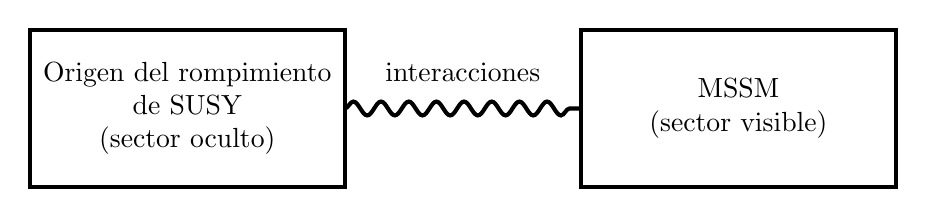
\begin{tikzpicture}

  \draw[line width=1.5] (0,0) rectangle (4,2) node[midway,align=center] (r1) {Origen del rompimiento\\ de SUSY\\ (sector oculto)};
  \draw[line width=1.5] (7,0) rectangle (11,2) node[midway, align=center] (r2) {MSSM\\ (sector visible)} ;

  \draw[line width=1.5,decorate,decoration={snake}] (4,1) -- (7,1) node[midway,above=.2cm] {interacciones};

\end{tikzpicture}

  \caption{Esquema de la supuesta estructura del rompimiento de supersimetría.}\label{fig:susy_breaking}
\end{figure}

Existen muchas propuestas de como estas interacciones mediadores pueden ser. Una
de ellas (e históricamente la más popular) es que estas interacciones son
gravitacionales (mSUGRA).

%% Más precisamente
%% estas asociados con la nueva física, incluyendo a la gravedad, que
%% aparece cerca de la escala de Planck. En este escenario

Una segunda posibilidad es que estas interacciones mediadores sean las
interacciones de gauge electrodébiles y QCD ordinarias. En estos escenarios
donde el rompimiento de supersimetría esta mediado por campos de gauge
(\emph{Gauge-mediated supersymmetry breaking} ó GMSB), los términos soft del
MSSM provienen de diagramas a un loop que involucran algunas partículas
mensajeras.

Si tenemos en cuenta a la gravedad, SUSY tiene que ser promovida a una simetría
local. Esta teoría supersimétrica local es llamada \emph{supergravedad}. Esto
unifica necesariamente las simetrías espacio-temporales ordinarias de la
Relatividad General con las transformaciones locales supersimétricas. En esta
teoría, el graviton de espín 2, tiene un supercompa\~nero fermión de espín 3/2
llamado \emph{gravitino}. Mientras la supersimetría no esté rota, el gravitón y
el gravitino son no masivos con dos estados de helicidad de espín. Una vez que
SUSY es espontáneamente rota, el gravitino adquiere una masa absorbiendo el
goldstino, que se convierte en sus componentes longitudinales (helicidad $\pm
1/2$). Este mecanismo es llamado \emph{super-Higgs}, y es el análogo al
mecanismo de Higgs ordinario de las teorías de gauge, donde los bosones de gauge
$W^\pm$ y $Z^0$ en el {\SM} adquieren masa absorbiendo los bosones de
Nambu-Goldstone asociados con la invarianza de gauge electrodébil
espontáneamente rota. La masa del gravitino es tradicionalmente llamada
$m_{3/2}$, y puede ser estimada como

\begin{equation}
  m_{3/2} \sim \avg{F} / M_P
\end{equation}
%
donde $F$ esta relacionada a la escala del rompimiento de SUSY. Esto implica
distintos valores esperados para la masa del gravitino dependiendo el modelo de
mediadores propuesto. En modelos de mediación por gravedad, la masa del
gravitino es comparable a la masa de las partículas del MSSM, por lo tanto es
esperado que sea de al menos el orden de 100 \gev. Sus interacciones van a ser
de intensidad gravitacional, el gravitino no juega ningún rol en física de
colisionadores, pero puede ser importante en cosmología.

En contraste, los modelos GMSB predicen un gravitino mucho más liviano que las
spartículas del MSSM.%% si $M_\text{mess} \ll M_P$.
En este caso, el gravitino es
la LSP, y todas las sparticulas del MSSM van a decaer eventualmente en un estado
final que incluye al gravitino.


%------
% GMSB
%------
\subsection{GMSB y GGM} %%Modelos de rompimiento de supersimetría mediados por campos de Gauge}

En los modelos de rompimiento de la supersimetría mediado por campos de gauge ó
GMSB, las interacciones ordinarias de gauge son las responsables de la aparición
del rompimiento soft de la supersimetría en el MSSM.

%% La idea básica es introducir
%% nuevos supermultipletes quirales, llamados mensajeros, que se acoplen ...
%% \note{Referencia: arxiv:9801271}

La mediación por campos de gauge es una de las maneras más simples y robustas
para transmitir el rompimiento de SUSY al MSSM. A pesar de su simpleza, existe
un gran número de modelos de GMSB. Para poder hacer un análisis fenomenológico
dentro del marco de GMSB de una forma no tan dependiente del modelo, pero con un
correcta base teórica, en \cite{GGM} se propone un marco lo más general posible
para describir los efectos de un sector oculto arbitrario, definiendo al
mecanismo de mediación por campos de gauge como: \emph{el límite en que las
  constantes de acoplamiento del MSSM $\alpha_i \to 0$, la teoría se desacopla
  en el MSSM y un sector oculto separado que rompe SUSY.}

A este marco general se lo conoce como \emph{General Gauge Mediation} ó GGM. El
conjunto de parámetros independientes de GGM esta compuesto por las tres masas
complejas de gauginos $M_1$, $M_2$ y $M_3$, y tres parámetros reales que
controlan las masas de los 5 sfermiones $m^2_{Q,U,D,L,E}$. Además los términos
trilineares $A$ siempre son pequeños.

Estos modelos ofrecen una rica variedad de estados finales en colisionadores
\cite{0911.4130}. La característica más destacable de estos modelos es el
gravitino liviano $m_{3/2} = M_\text{weak}$. La masa del gravitino en modelos
GGM es típicamente del orden del eV (en algunos casos puede llegar al \gev), lo
cual implica que el {\gravino} es la LSP. Esto asegura que los efectos de
mediación por campos de gauge domine por sobre la mediación por gravedad.

Uno de los aspectos teóricos interesantes de SUSY es que si esta simetría es
realizada como una simetría local, incorpora de forma necesaria y automática la
gravedad.
%% Esta conexión no tiene ninguna consecuencia en la mayor parte de la
%% fenomenología en colisionadores, porque las interacciones gravitatorias no son
%% relevantes. Sin embargo, esto no necesariamente cierto si el gravitino es muy
%% liviano.
%% El gravitino obtiene su masa absorbiendo el goldstino de espín 1/2 asociado al
%% rompimiento espontáneo de la supersimetría. En el límite de altas energías, las
%% interacciones de las componentes de helicidad $\pm 1/2$ del gravitino son las
%% mismas que las del goldstino.
%% Estas interacciones son proporcionales a $1/m_{\gravino}$ en el límite
%% $m_{\gravino} \to 0$ y son potencialmente importantes incluso para procesos a
%% energías ordinarias. Sin embargo, la intensidad de las interacciones del
%% gravitino no puede ser arbitrariamente grande.
La masa del gravitino esta relacionada con la escala del rompimiento de SUSY por,

\begin{equation}
  m_{\gravino} = \frac{\Lambda^2_{\text{SUSY}}}{\sqrt{3}M_P}
\end{equation}

La escala $\Lambda_{\text{SUSY}}$ tiene que ser al menos la masa de las
partículas supersimétricas más pesadas. Si consideramos que
$\Lambda_{\text{SUSY}} > 1 \tev$ entonces $m_{\gravino} > 10^{-4} \eV$.
Y por otro lado, los límites cosmológicos \cite{PhysRevLett.48.223,Moroi:1993mb}
bajo ciertas condiciones, ponen un límite superior $m_{\gravino} < 10^4 \eV$.%% , al menos en ausencia
%% de \hl{late inflation}.

El hecho de que la LSP sea siempre el gravitino, determina que la partícula mas
liviana del MSSM es entonces la NLSP, y siempre decae a un gravitino y su
compañero del SM. Como este decaimiento esta altamente suprimido por la escala
de rompimiento de SUSY, la NLSP puede decaer de forma inmediata (\emph{promtp}) o luego de haber
atravesado una cierta distancia en el detector. En lo que sigue sólo nos concentraremos
en decaimientos \emph{prompt}.
Esta supresión de la tasa de decaimiento también significa que todas las
spartículas pesadas decaen pasando por la NLSP antes de decaer en un gravitino.
Es por este motivo que la naturaleza de la NLSP es el aspecto más importante del
espectro de GMSB para los estados finales en colisionadores.


La topología típica de un evento GGM esta ilustrada en la
\cref{fig:ggm_event}, en la cual se pueden observar varias caracteristicas
importantes. El gravitino siempre va a escapar del detector, dejando una
cantidad significativa de energía faltante. Mientras tanto, el compañero del SM
va a tender a ser central y energético (asumiendo que la NLSP decae dentro del
detector), ya que es en general mucho más liviano que la NLSP. Dado que en cada
evento SUSY se producen dos NLSPs, es claro que las partículas producidas en un
colisionador van a estar determinadas por la naturaleza de la NLSP.

\begin{figure}[!htbp]
  \centering
  %%\includegraphics[width=0.5\textwidth]{figures/ggm_event}
  %\usetikzlibrary{positioning}
\usetikzlibrary{arrows}
\usetikzlibrary{patterns}
\usetikzlibrary{decorations.markings}
\usetikzlibrary{calc}
\usetikzlibrary{decorations}
\usetikzlibrary{decorations.pathmorphing}


\makeatletter

% gluon decoration (based on the original coil decoration)
\pgfdeclaredecoration{coilgluon}{coil}
{
  \state{coil}[switch if less than=%
    0.5\pgfdecorationsegmentlength+%>
    \pgfdecorationsegmentaspect\pgfdecorationsegmentamplitude+%
    \pgfdecorationsegmentaspect\pgfdecorationsegmentamplitude to last,
    width=+\pgfdecorationsegmentlength]
        {
          \pgfpathcurveto
              {\pgfpoint@oncoil{0    }{ 0.555}{1}}
              {\pgfpoint@oncoil{0.445}{ 1    }{2}}
              {\pgfpoint@oncoil{1    }{ 1    }{3}}
              \pgfpathcurveto
                  {\pgfpoint@oncoil{1.555}{ 1    }{4}}
                  {\pgfpoint@oncoil{2    }{ 0.555}{5}}
                  {\pgfpoint@oncoil{2    }{ 0    }{6}}
                  \pgfpathcurveto
                      {\pgfpoint@oncoil{2    }{-0.555}{7}}
                      {\pgfpoint@oncoil{1.555}{-1    }{8}}
                      {\pgfpoint@oncoil{1    }{-1    }{9}}
                      \pgfpathcurveto
                          {\pgfpoint@oncoil{0.445}{-1    }{10}}
                          {\pgfpoint@oncoil{0    }{-0.555}{11}}
                          {\pgfpoint@oncoil{0    }{ 0    }{12}}
        }
        \state{last}[next state=final]
              {
                \pgfpathcurveto
                    {\pgfpoint@oncoil{0    }{ 0.555}{1}}
                    {\pgfpoint@oncoil{0.445}{ 1    }{2}}
                    {\pgfpoint@oncoil{1    }{ 1    }{3}}
                    \pgfpathcurveto
                        {\pgfpoint@oncoil{1.555}{ 1    }{4}}
                        {\pgfpoint@oncoil{2    }{ 0.555}{5}}
                        {\pgfpoint@oncoil{2    }{ 0    }{6}}
              }
              \state{final}{}
}

\def\pgfpoint@oncoil#1#2#3{%
  \pgf@x=#1\pgfdecorationsegmentamplitude%
  \pgf@x=\pgfdecorationsegmentaspect\pgf@x%
  \pgf@y=#2\pgfdecorationsegmentamplitude%
  \pgf@xa=0.083333333333\pgfdecorationsegmentlength%
  \advance\pgf@x by#3\pgf@xa%
}

\makeatother

\tikzset{
  proton/.style={line width=1pt,preaction={preaction={draw,line width=5pt},draw,white,line width=3pt}},
  photon/.style={decorate, decoration={snake}, draw=black},
  higgs/.style={draw, dashed},
  fermion/.style={draw=black, postaction={decorate},decoration={markings}},
  gluon/.style ={decorate, decoration={coilgluon,amplitude=4pt, segment length=5pt}},
  gluino/.style={decorate, decoration={coilgluon,amplitude=4pt, segment length=5pt}, preaction={draw}},
  vertex/.style={draw,shape=circle,fill=black,minimum size=0pt,inner sep=0pt},
}

%% \semiloop[fermion][<draw options>]{<first node>}{<second node>}{<angle>}[<label>][<below, default: above>];
%% \NewDocumentCommand\semiloop{O{black}mmmO{}O{above}}
%% {%
%%   \draw[#1] let \p1 = ($(#3)-(#2)$) in (#3) arc (#4:({#4+180}):({0.5*veclen(\x1,\y1)})node[midway, #6] {#5};)
%% }

\colorlet{red}{red!60}
\colorlet{blue}{blue!60}
\colorlet{green}{green!60}
\colorlet{blue}{blue!50!black!70}
\colorlet{green}{green!50!black!70}
\colorlet{purple}{purple!90!black!70}
\colorlet{gray1}{black!10}

\tikzset{
    arr/.style={line width=1,
      decoration={markings,mark=at position 1 with {\arrow[scale=1.5]{>}}},
      postaction={decorate}
      },
    rec/.style={rectangle,
                fill, black,
                fill=gray1,
                very thick,
                text width=2.7cm,
                minimum height=1.5cm,
                text centered}
}


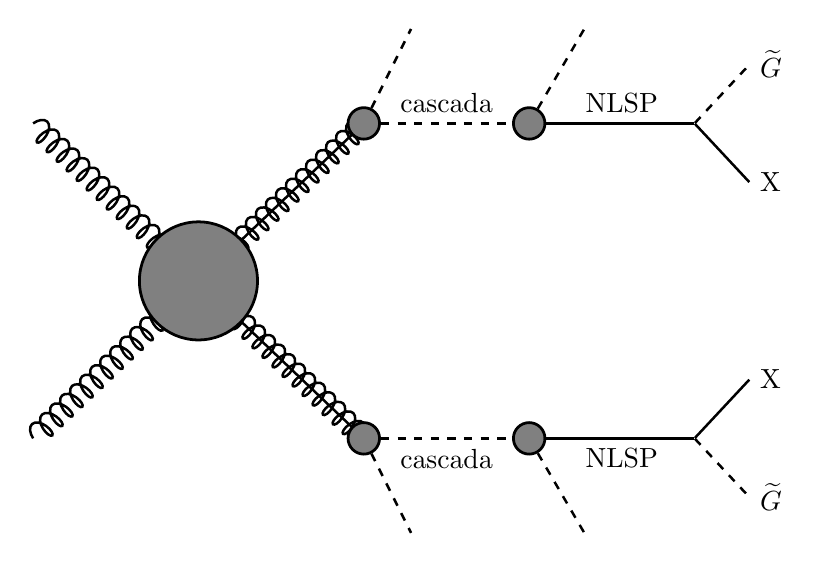
\begin{tikzpicture}

	\tikzset{
    		line/.style={line width=0.9},
    		dline/.style={dashed,line width=0.9},
  	}

	\definecolor{blue1}{HTML}{3F66BD}
	\definecolor{blue2}{HTML}{2C4784}

	\coordinate[vertex] (O) at (0,0);

	\coordinate[vertex] (C1) at (2.1, 2);
	\coordinate[vertex] (C2) at (2.1,-2);

	\coordinate[vertex] (N1_a) at (4.2, 2);
	\coordinate[vertex] (N2_a) at (4.2,-2);

	\coordinate[vertex] (N1_b) at (6.3, 2);
	\coordinate[vertex] (N2_b) at (6.3,-2);

	\coordinate[vertex] (G1) at (7, 2.75);
	\coordinate[vertex] (X1) at (7, 1.25);

	\coordinate[vertex] (G2) at (7,-2.75);
	\coordinate[vertex] (X2) at (7,-1.25);

	\draw[line,gluon] (-2.1,-2) -- (O);
	\draw[line,gluon] (-2.1, 2) -- (O);

	\draw[line] (O) -- (C1);
	\draw[line] (O) -- (C2);
	\draw[line,gluino] (O) -- (C1);
	\draw[line,gluino] (O) -- (C2);

	\draw[line] (4.0, 2) -- (N1_b) node[above, pos=.6] {NLSP};
	\draw[line] (4.0,-2) -- (N2_b) node[below, pos=.6] {NLSP};

	\draw[dline] (N1_b) -- (G1) node[right] {$\widetilde{G}$};
	\draw[line] (N1_b) -- (X1) node[right] {X};

	\draw[dline] (N2_b) -- (G2) node[right] {$\widetilde{G}$};
	\draw[line] (N2_b) -- (X2) node[right] {X};

    	\draw[black, line width=1, fill=gray] (O) circle (0.75cm); 

  	\draw[dline,fill=white] (C1) -- (N1_a) node[black,above,pos=.5] {cascada};
  	\draw[dline,fill=white] (C2) -- (N2_a) node[black,below,pos=.5] {cascada};

	\draw[dline] (C1) -- (2.7, 3.2);
	\draw[dline] (C2) -- (2.7,-3.2);
	\draw[dline] (N1_a) -- (4.9, 3.2);
	\draw[dline] (N2_a) -- (4.9,-3.2);


	\draw[black, line width=1,fill=gray] (C1) circle (0.20cm);
	\draw[black, line width=1,fill=gray] (C2) circle (0.20cm);
	\draw[black, line width=1,fill=gray] (N1_a) circle (0.20cm);
	\draw[black, line width=1,fill=gray] (N2_a) circle (0.20cm);

\end{tikzpicture}

  \caption{Esquema de la topología típica de un evento GGM en un colisionador de hadrones.
    En la interaccion fuerte se produce un par de gluinos que luego decaen en forma de cascada,
    hasta llegar a la NLSP, que decae en un gravitino {\gravino} y su companero del SM ($X$). Los
    gravitinos escapan el detector dejando un gran cantidad de energia faltante.}
  \label{fig:ggm_event}
\end{figure}


%%\subsection{Gravitino LSP}

%% Como resultado del rompimiento espontaneo de la supersimetria,
%% el espectro fisico contiene un fermion no masivo de spin 1/2,
%% el goldstino. Cuando la teoria supersimetrica global esta acoplada
%% a la gravedad y promocionada a una teoria supersimetrica local,
%% el goldstino provee los modos longitudinales de spin 3/2 del graviton:
%% el gravitino.
%% Como resultado de este mecanismo de super-Higgs, el gravitino adquiere una masa
%% que bajo la condicion de la anulacion de la constante cosmologica esta dada por:

%% \begin{equation}
%%   m_{3/2} = \frac{F_0}{\sqrt{3}M_P}
%% \end{equation}
%% %
%% donde $M_P = (8\pi G_N)^{-1/2} = 2.4 \times 10^{18} \gev$ es la masa reducida de Planck.
%% Y $F_0$ es la contribucion total del VEV de rompimiento de SUSY de los campos auxiliares
%% normalizado de tal forma que la energia de vacio de la teoria supersimetrica global es
%% $V = F_0^2$...

%% En los modelos GMSB, el gravitino es la particula supersimetrica más liviana (LSP) para
%% cualquier valor relevante de $F$. Si la paridad-R es conservada, todas las particulas
%% supersimetricas van a seguir cadenas de decaimineto que terminan en gravitinos.

%% There is then still a window of
%% perhaps 9 orders of magnitude for the mass of a light gravitino. In particular classes of models,
%% this window can be much smaller. Throughout this window, mG˜ is clearly insignificant for
%% collider kinematics, and so can be taken to simply parameterize the strength of the gravitino’s
%% interactions.


\subsubsection{La NLSP}

Como se ha mencionado, la segunda partícula supersimétrica más liviana (NLSP) juega un rol fundamental
en la fenomenología de los modelos GGM. Suponiendo que se conserva la paridad-R,
todas las partículas supersimétricas van a decaer rápidamente en una cascada
hasta la NLSP, y esta va a decaer en un gravitino y una partícula del SM. Por este motivo, la
naturaleza de la NLSP determina los diferentes estados finales en los
colisionadores así como también algunas propiedades cosmológicas. En principio
la NLSP puede ser cualquier particula del MSSM dependiendo de la elección de los
parámetros del modelo. Para la mayor parte del espacio de parametros será el neutralino ó
el stau, y para algunas regiones muy restrictivas, el
sneutrino\cite{arxiv:9801271}.
Las partículas, que aunque no son NLSP, tienen un decaimiento dominante en su
compañero supersimetrico y el {\gravino} se denominan co-NLSP.

%% En el caso de que sea neutralino, esta tiene, en la mayoria de los
%% casos, una componente dominante de bino, ya que el cociente $\mu/\M{1}$
%% es generalemente mayor a 1. %Una excepcion ocurre para N grande y M y lambda
%chico?

%% Las tazas de decaimiento del {\ninoone} NLSP son:\note{pongo las formulas?}

%% \begin{align}
%%   \Gamma (\ninoone \to \gamma \gravino) =
%% \end{align}

%% Para
%% valores grandes de $\tan \beta$, las dos primeras generaciones de sleptones
%% decaen como $\susy{\ell}_R \to \ell \tau \stau$ y el stau es la ``única'' NLSP.
%% Otra posibilidad es que el
%% {\ninoone}, aunque no sea la NLSP, esta degenerado en masa con el
%% {\stau}, y su decaimiento dominante sea a un fotón y un
%% goldstino. En este caso {\stau} y {\ninoone} son co-NLSP.

%% La posibilidad de que el sneutrino sea NLSP es muy marginal. Requiere
%% valores de $N$ tan grandes y valores tan chicos de $\Lambda$ que el
%% descubrimiento de SUSY debería darse muy pronto. En este caso el
%% sneutrino decae en un neutrino y un goldstino.

Todos estos casos corresponden a una fenomenología completamente diferente en
los experimentos de altas energías.


\subsubsection{Neutralino NLSP}

Como se detalla en la \cref{sec:mass_NC}, los auto-estados de masa de los
neutralinos dependen de cuatro parámetros: $M_1$, $M_2$, $\mu$ y $\tan\beta$.
Dependiendo los valores de estos cuatro parámetros, el decaimiento dominante
sera distinto. Como el espacio de parámetros del neutralino es de cuatro
dimensiones, resulta difícil hacer un estudio detallado de la fenomenología asociada.
En general se estudian algunos límites simplificados, donde el neutralino
es básicamente uno de los auto-estados de gauge puro, es decir, es puramente
bino, wino o higgsino. %%\note{Agregar referencias}

El neutralino NLSP decae a $X + \gravino$ donde $X=\gam,Z,h$, y los distintos
auto-estados de gauge se caracterizan por tener distintos BR a los diferentes $X$
\cite{Ruderman:2011vv}.
Los binos decaen a fotones con un BR $\sim \cos^2\theta_W$, con una componente
menor a $Z$'s, con BR $\sim \sin^2\theta_W$ (ver figura
\cref{fig:bino_wino_br}). Por otro lado estos BR se intercambian en el caso de
que la NLSP sea el wino neutro, que decae mayormente a $Z$'s. Si la NLSP es
higgsino, este decae en forma dominante a $Z$ ó $h$, con BR que depende en el
valor de $\tan\beta$ y del signo de $\mu$. Hay tres casos: (i) el decaimiento
del higgsino es preferentemente a $Z$ para bajo $\tan\beta$ y $\mu$ positivo,
(ii) mayormente a $h$ para bajo $\tan\beta$ y $\mu$ negativo, y (iii) una mezcla
de $Z$ y $h$ a moderado y alto $\tan\beta$.

\begin{figure}[h]
  \centering
  %\includegraphics[width=0.9\textwidth]{figures/bino_wino_br}

  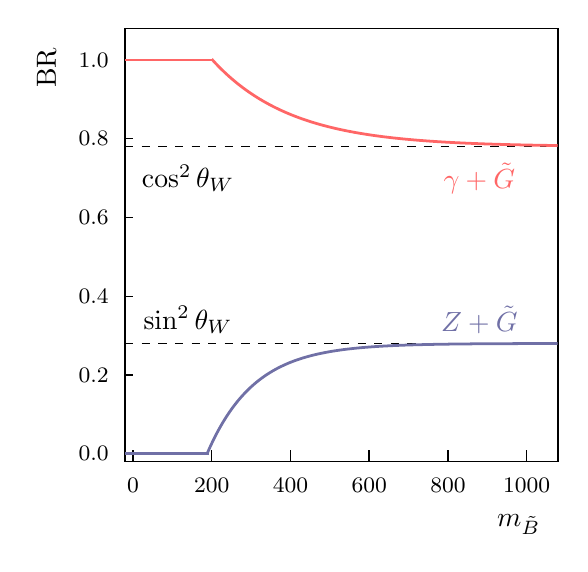
\begin{tikzpicture}

    \tikzstyle{region} = [rounded corners, fill, opacity=0.5, line width=0.1, green]
    \tikzstyle{axis} = [line width=0.6]
    \tikzstyle{tick} = [line width=0.5]
    \tikzstyle{point} = [blue, fill=blue!20]


    \draw[axis] (0,0) -- (5.5,0) node at (5.0,-0.8) {$m_{\tilde{B}}$};
    \draw[axis] (0,0) -- (0,5.5) node[rotate=90] at (-1,5.0) {BR};

    \draw[axis] (5.5,0) -- (5.5,5.5);
    \draw[axis] (0,5.5) -- (5.5,5.5);

    \draw[dashed] (0,1.5) -- (5.5,1.5) node[baseline=left] at (0.8, 1.8) {$\sin^2 \theta_W$};
    \draw[dashed] (0,4.0) -- (5.5,4.0) node[baseline=left] at (0.8, 3.6) {$\cos^2 \theta_W$};


    \draw[tick] (0,5.1) -- (0.1,5.1) node at (-0.4, 5.1) {\footnotesize 1.0};
    \draw[tick] (0,4.1) -- (0.1,4.1) node at (-0.4, 4.1) {\footnotesize 0.8};
    \draw[tick] (0,3.1) -- (0.1,3.1) node at (-0.4, 3.1) {\footnotesize 0.6};
    \draw[tick] (0,2.1) -- (0.1,2.1) node at (-0.4, 2.1) {\footnotesize 0.4};
    \draw[tick] (0,1.1) -- (0.1,1.1) node at (-0.4, 1.1) {\footnotesize 0.2};
    \draw[tick] (0,0.1) -- (0.1,0.1) node at (-0.4, 0.1) {\footnotesize 0.0};

    \draw[tick] (5.1,0) -- (5.1,0.15) node at (5.1,-0.3) {\footnotesize 1000};
    \draw[tick] (4.1,0) -- (4.1,0.15) node at (4.1,-0.3) {\footnotesize 800};
    \draw[tick] (3.1,0) -- (3.1,0.15) node at (3.1,-0.3) {\footnotesize 600};
    \draw[tick] (2.1,0) -- (2.1,0.15) node at (2.1,-0.3) {\footnotesize 400};
    \draw[tick] (1.1,0) -- (1.1,0.15) node at (1.1,-0.3) {\footnotesize 200};
    \draw[tick] (0.1,0) -- (0.1,0.15) node at (0.1,-0.3) {\footnotesize 0};

    \draw[blue, line width=1] (0,0.1) -- (1.06,0.1);
    \draw[blue,line width=1] plot[domain=1.04:5.5, samples=500] ({\x},{1.5*(1 - exp(-((\x-1)/0.6)))});

    \draw[red, line width=1] (0,5.1) -- (1.1,5.1);
    \draw[red,line width=1] plot[domain=1.1:5.5, samples=500] ({\x},{4.+1.5*(exp(-((\x-0.8)/1)))});

    \node[blue] at (4.5, 1.8) {$Z+ \tilde{G}$};
    \node[red]  at (4.5, 3.6) {$\gamma + \tilde{G}$};
\end{tikzpicture}

  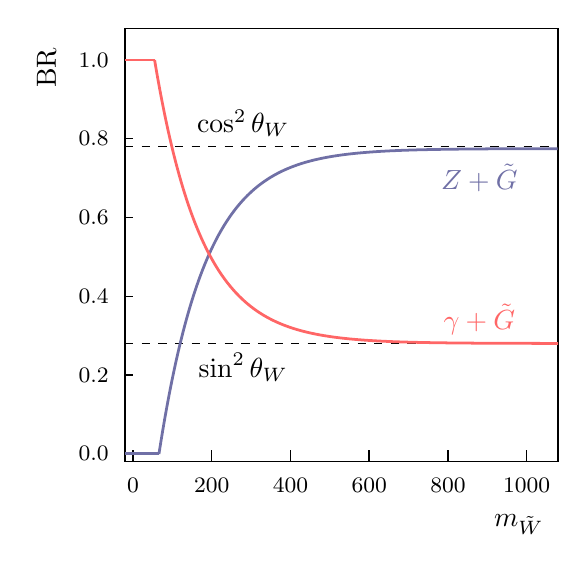
\begin{tikzpicture}

    \tikzstyle{region} = [rounded corners, fill, opacity=0.5, line width=0.1, green]
    \tikzstyle{axis} = [line width=0.6]
    \tikzstyle{tick} = [line width=0.5]
    \tikzstyle{point} = [blue, fill=blue!20]

    \draw[axis] (0,0) -- (5.5,0) node at (5.0,-0.8) {$m_{\tilde{W}}$};
    \draw[axis] (0,0) -- (0,5.5) node[rotate=90] at (-1,5.0) {BR};

    \draw[axis] (5.5,0) -- (5.5,5.5);
    \draw[axis] (0,5.5) -- (5.5,5.5);

    \draw[dashed] (0,1.5) -- (5.5,1.5) node[baseline=left] at (1.5, 1.2) {$\sin^2 \theta_W$};
    \draw[dashed] (0,4.0) -- (5.5,4.0) node[baseline=left] at (1.5, 4.3) {$\cos^2 \theta_W$};


    \draw[tick] (0,5.1) -- (0.1,5.1) node at (-0.4, 5.1) {\footnotesize 1.0};
    \draw[tick] (0,4.1) -- (0.1,4.1) node at (-0.4, 4.1) {\footnotesize 0.8};
    \draw[tick] (0,3.1) -- (0.1,3.1) node at (-0.4, 3.1) {\footnotesize 0.6};
    \draw[tick] (0,2.1) -- (0.1,2.1) node at (-0.4, 2.1) {\footnotesize 0.4};
    \draw[tick] (0,1.1) -- (0.1,1.1) node at (-0.4, 1.1) {\footnotesize 0.2};
    \draw[tick] (0,0.1) -- (0.1,0.1) node at (-0.4, 0.1) {\footnotesize 0.0};

    \draw[tick] (5.1,0) -- (5.1,0.15) node at (5.1,-0.3) {\footnotesize 1000};
    \draw[tick] (4.1,0) -- (4.1,0.15) node at (4.1,-0.3) {\footnotesize 800};
    \draw[tick] (3.1,0) -- (3.1,0.15) node at (3.1,-0.3) {\footnotesize 600};
    \draw[tick] (2.1,0) -- (2.1,0.15) node at (2.1,-0.3) {\footnotesize 400};
    \draw[tick] (1.1,0) -- (1.1,0.15) node at (1.1,-0.3) {\footnotesize 200};
    \draw[tick] (0.1,0) -- (0.1,0.15) node at (0.1,-0.3) {\footnotesize 0};

    \draw[blue, line width=1] (0,0.1) -- (0.43,0.1);
    \draw[blue,line width=1] plot[domain=0.43:5.5, samples=500] ({\x},{1.5*(2.65 - exp(-((\x-1)/0.6)))});

    \draw[red, line width=1] (0,5.1) -- (0.38,5.1);
    \draw[red,line width=1] plot[domain=0.375:5.5, samples=500] ({\x},{1.5+1.5*(exp(-((\x-0.9)/0.6)))});

    \node[blue] at (4.5, 3.6) {$Z+ \tilde{G}$};
    \node[red]  at (4.5, 1.8) {$\gamma + \tilde{G}$};
\end{tikzpicture}


  \caption{Tasas de decaimiento del neutralino más liviano a gravitino más fotones o bosones $Z$ en funcion de la masa del mismo. En la izquierda
    el caso que el neutralino es puramente bino, y a la derecha puramente wino.}
  \label{fig:bino_wino_br}
\end{figure}

Cuando la NLSP es mayormente wino, hay una muy pequeña degeneración entre el
wino neutro y el cargado. Cuando esto pasa, el decaimiento de tres cuerpos al
wino neutro comienza a ser excluido, y el wino cargado prefiere decaer
directamente a $W^{\pm}$ y un gravitino. En otras palabras, el wino neutro y el
wino cargado se vuelve co-NLSPs, y los estados finales van a contener $W$'s,
$Z$'s y fotones.

Como en cada evento de SUSY hay un par de neutralinos, los estados
finales involucrarán una combinación de pares de $\gam + \gravino$, $Z +
\gravino$ y $h + \gravino$. Adicionalmente, si hay una diferencia chica entre la masa
del neutralino y del chargino más liviano, puede haber cadenas de decaimiento
que terminen en $W^\pm + \gravino$.

El escenario más estudiado y más buscado es cuando la NLSP es un neutralino
puramente bino. En este caso el estado final consiste en $\gam\gam + \met$.
Sin embargo en el caso más general de neutralino NLSP, aparecen muchas otros
canales menos explorados que involucran leptones, $Z$, $W$, jets y higgses de
alto {\pt} y energía faltante.

%% Por otro lado, la degeneración\'on entre los higgsinos cargados y
%% neutros es generalmente mayor, de modo que solo el neutralino mas
%% livinao decae directamente en gravitino.

En el caso en el cual el neutralino es una mezcla mayoritaria de bino y higgsino, el
estado final dependerá del parámetro de masa del higgsino $\mu$. Si
$\mu <0$, el estado final de la cascada va a tener una gran contribución
de $\ninoone \to h\gravino$ donde el Higgs decaerá mayormente a $h\to b \bar{b}$,
dejando un estado final con un fotón, b-jets y {\met}. En el escenario donde
$\mu>0$ el decaimiento dominante estará compartido entre $\ninoone \to \gam\gravino$
y $\ninoone\to Z \gravino$, y el decaimiento a Higgs estara suprimido,
dando como estado final un fotón, múltiples jets (incluyendo
los dos del decaimiento de $Z$) y {\met}.

Esta Tesis se centrará en este ultimo caso. En el \cref{cap:simulaciones}
se describirá en detalle el modelo de se\~nal que motiva el estado final
de el presente análisis.


%% Esta Tesis se centrara en un neutralino NLSP que es una mezcla mayoritaria
%% de bino y higgsino, donde la probabilidad de decaimiento en fotones y $Z$
%% es similar y esta suprimido el decaimiento a Higgs, dejando como estado
%% final un único fotón, jets, y energía faltante.


\subsection{Producción de partículas supersimétricas}

En la \cref{fig:xs_lhc_8tev} se puede ver la sección eficaz para la producción
de squarks y gluinos en el LHC comparada para los distintos canales de
producción. La producción por interacción fuerte es mucho mayor a la de
spartículas que interactúan débilmente, y por esta razón la mayoría de las
búsquedas se basan en la producción de gluinos y squarks.

\begin{figure}[!htbp]
  \centering
  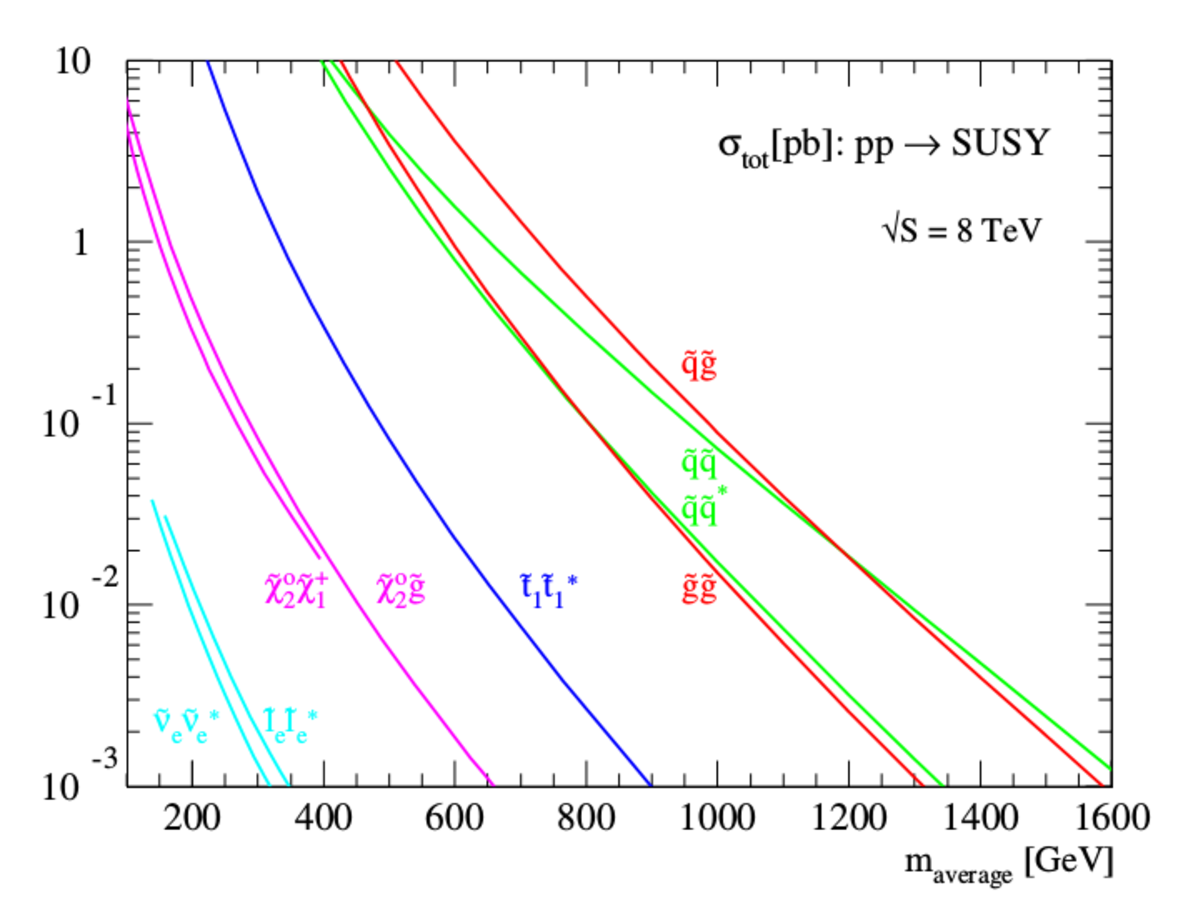
\includegraphics[width=0.8\textwidth]{figures/susy_lhc_xs_8tev}
  \caption{Sección eficaz de producción de partículas supersimétricas, como
    función de su masa, para los distintos canales de producción en el LHC con
    $\sqrt{s} = 8 \tev$ calculada a NLO usando \prospino.}
  \label{fig:xs_lhc_8tev}
\end{figure}


En los colisionadores hadrónicos, las partículas supersimétricas pueden ser
producidas de a pares a partir de colisiones de interacción
electrodébil (ver \cref{fig:ewkprod}):

\begin{align}
  &q\bar{q} \quad \to \quad \chinop \chinom, \nino \nino \label{eq:qq_ewk} \\
  &q\bar{q} \quad \to \quad \susy{\ell}^{+}_{i}\susy{\ell}^{-}_{j}, \susy{\nu}_{\ell}\susy{\nu}^{*}_{\ell} \label{eq:qq_ewk2}
\end{align}
%
y a partir de interacciones fuertes (ver \cref{fig:strongprod1,fig:strongprod2}):

\begin{align}
  gg \quad &\to \quad \gluino\gluino, \susy{q_i}\susy{q_j}^{*}, \label{eq:gg} \\
  gq \quad &\to \quad \gluino\susy{q_i}, \label{eq:gq} \\
  q\bar{q} \quad &\to \quad \gluino\gluino, \susy{q_i}\susy{q_j}^{*}, \label{eq:qqbar} \\
  qq \quad &\to \quad \susy{q_i}\susy{q_j}, \label{eq:qq}
\end{align}

La producciones en \cref{eq:qq_ewk,eq:qq_ewk2} obtienen contribuciones de los
bosones vectoriales electrodébiles en el canal $s$, mientras que las de
\cref{eq:qq_ewk} también tienen contribuciones del canal $t$ que son menos
importantes en la mayoría de los modelos. Los procesos en
\cref{eq:gg,eq:gq,eq:qqbar,eq:qq} tienen contribuciones del intercambio del
correspondiente squark o gluino en el canal $t$, y \cref{eq:gg} y
\cref{eq:qqbar} también tienen contribuciones de gluones en el canal $s$.

\begin{figure}[!htbp]
  \centering 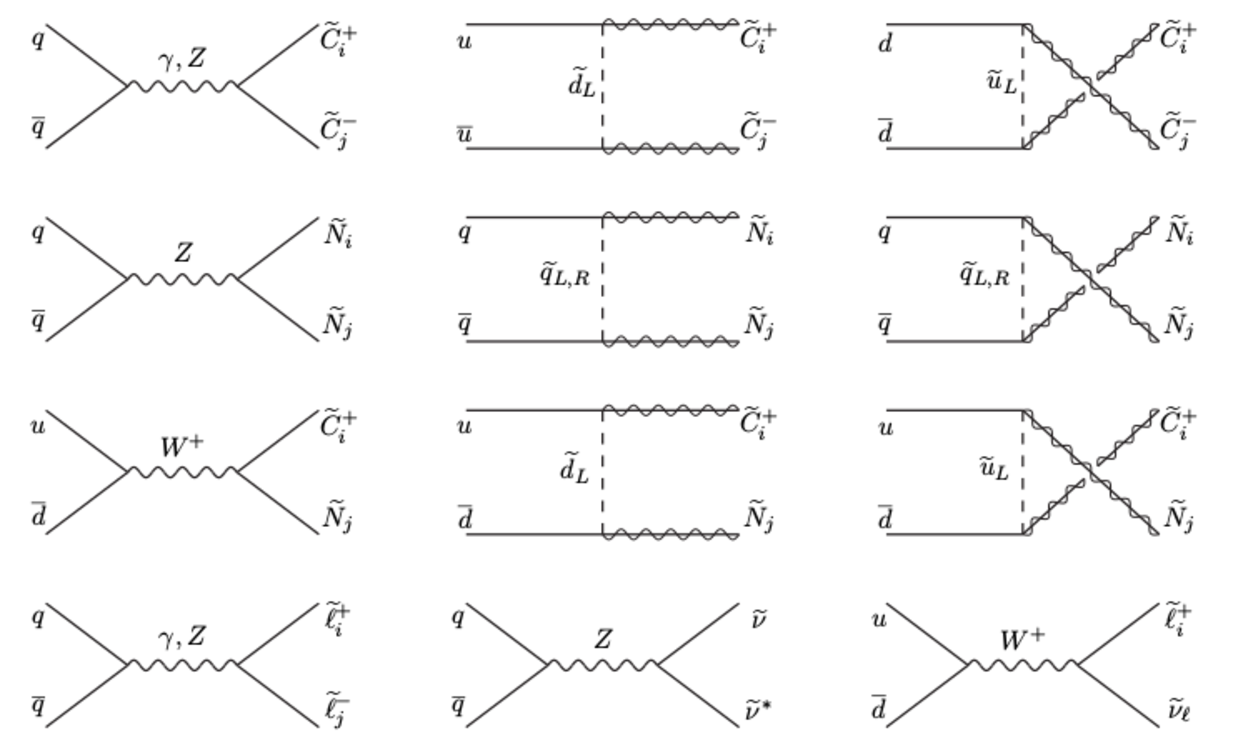
\includegraphics[width=0.6\textwidth]{figures/figure_101}
  \caption{Diagramas de Feynman para la producción electrodébil de spartículas
    en colisionadores de hadrones vía aniquilación quark-antiquark.}
  \label{fig:ewkprod}
\end{figure}

\begin{figure}[!htbp]
  \centering 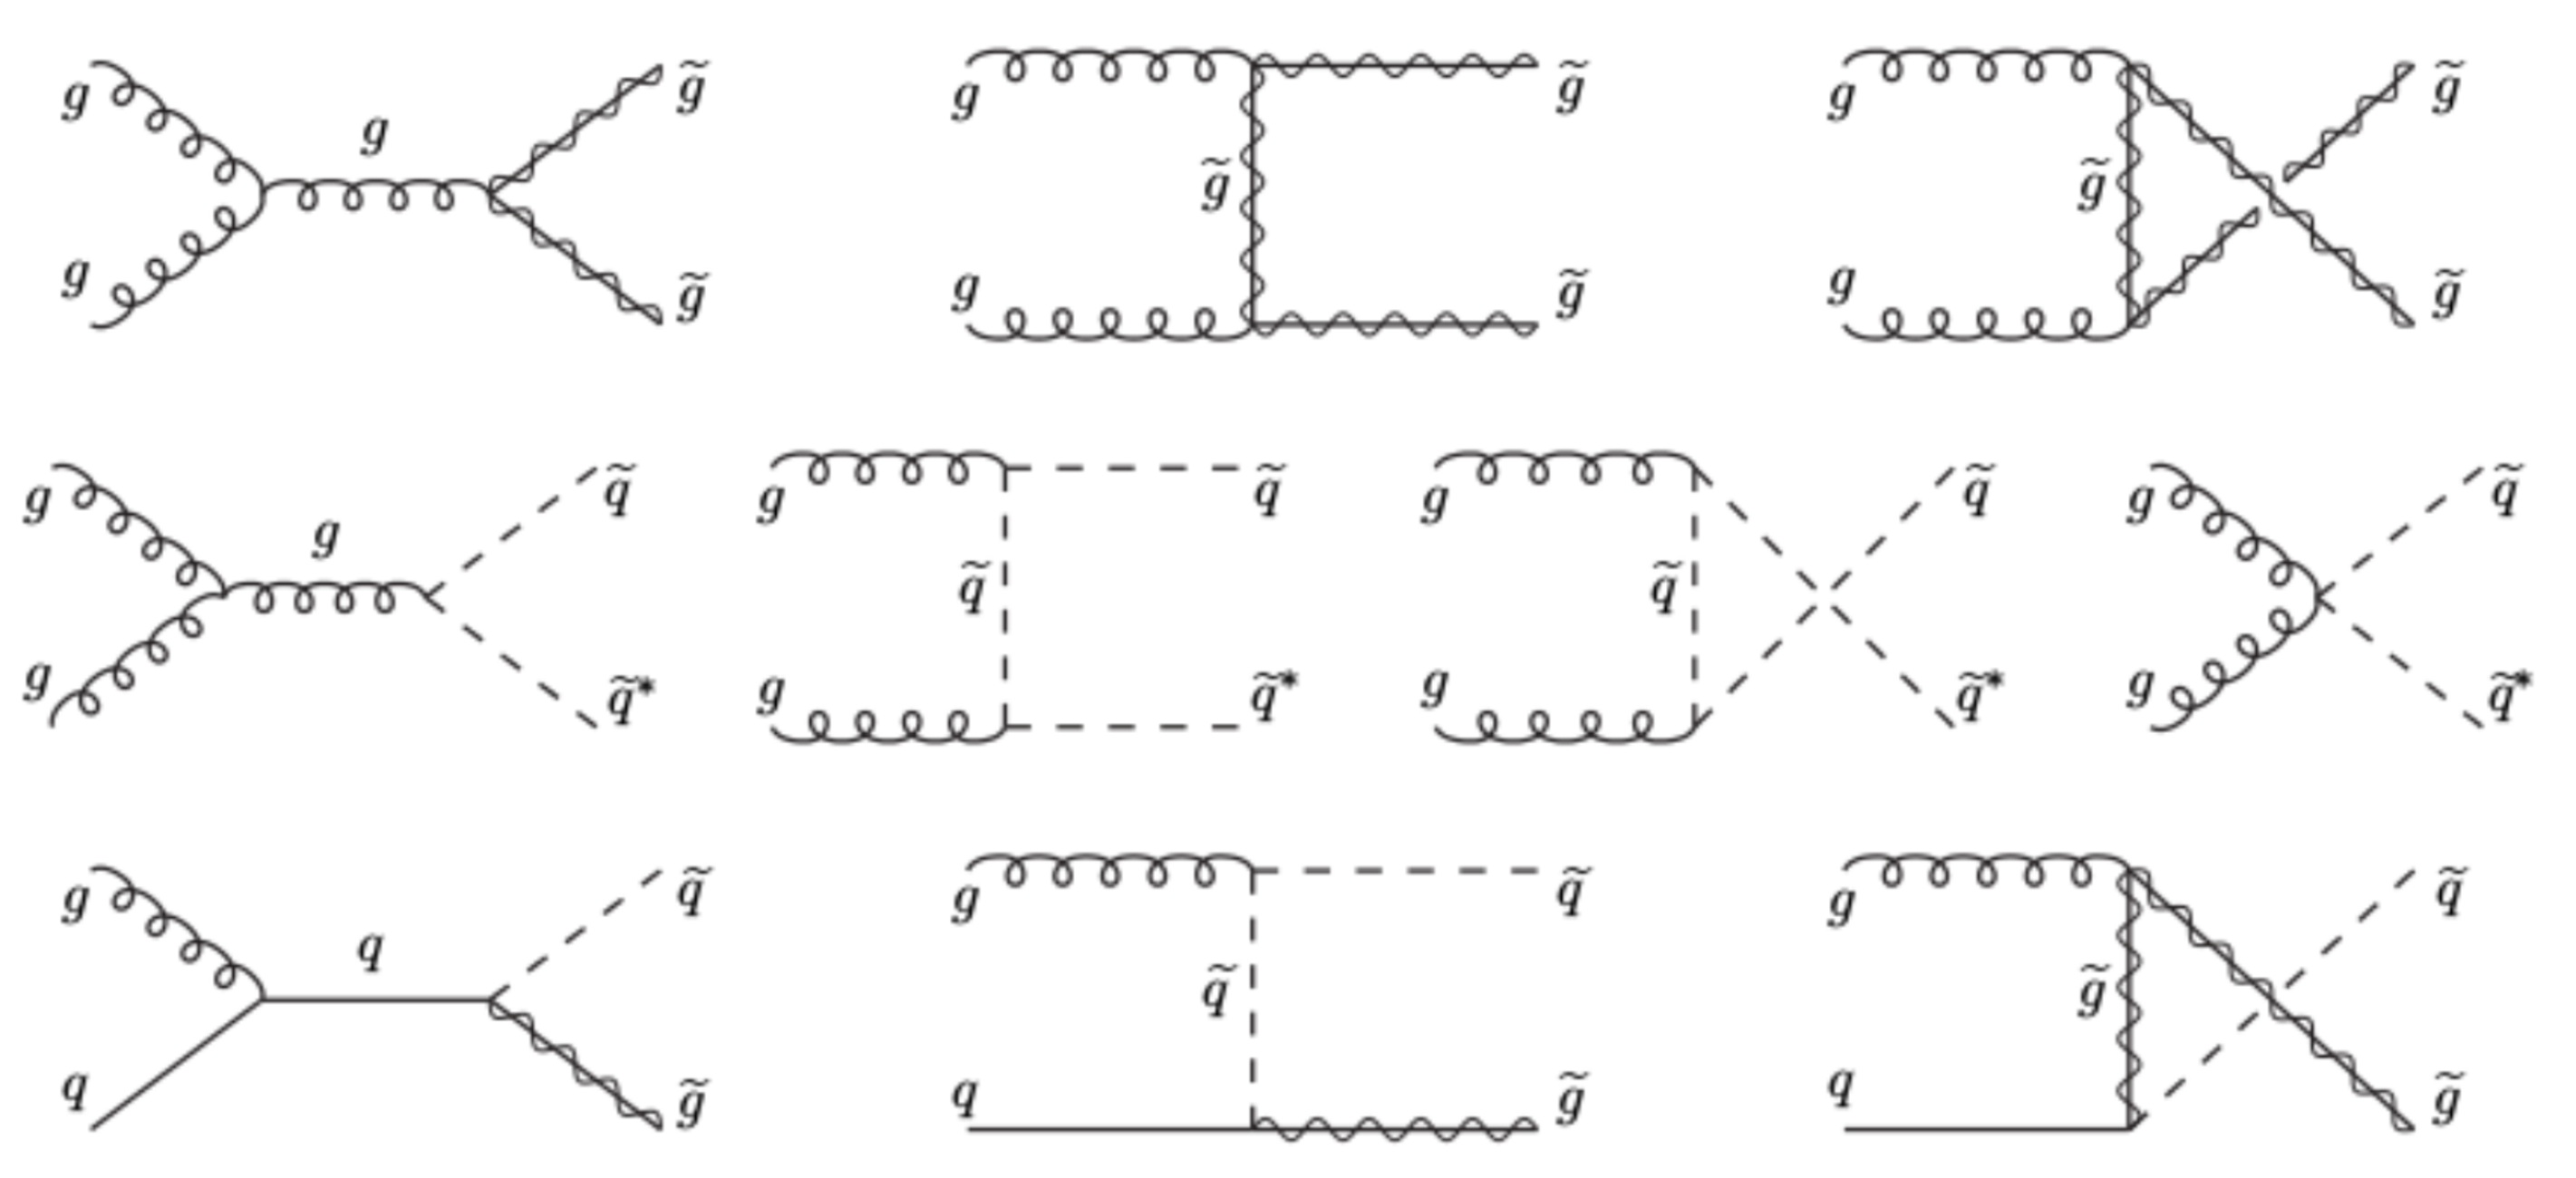
\includegraphics[width=0.6\textwidth]{figures/figure_102}
  \caption{Diagramas de Feynman para la producción de gluinos y squarks en
    colisionadores de hadrones vía fusión gluón-gluón y gluón squark.}
  \label{fig:strongprod1}
\end{figure}

\begin{figure}[!htbp]
  \centering 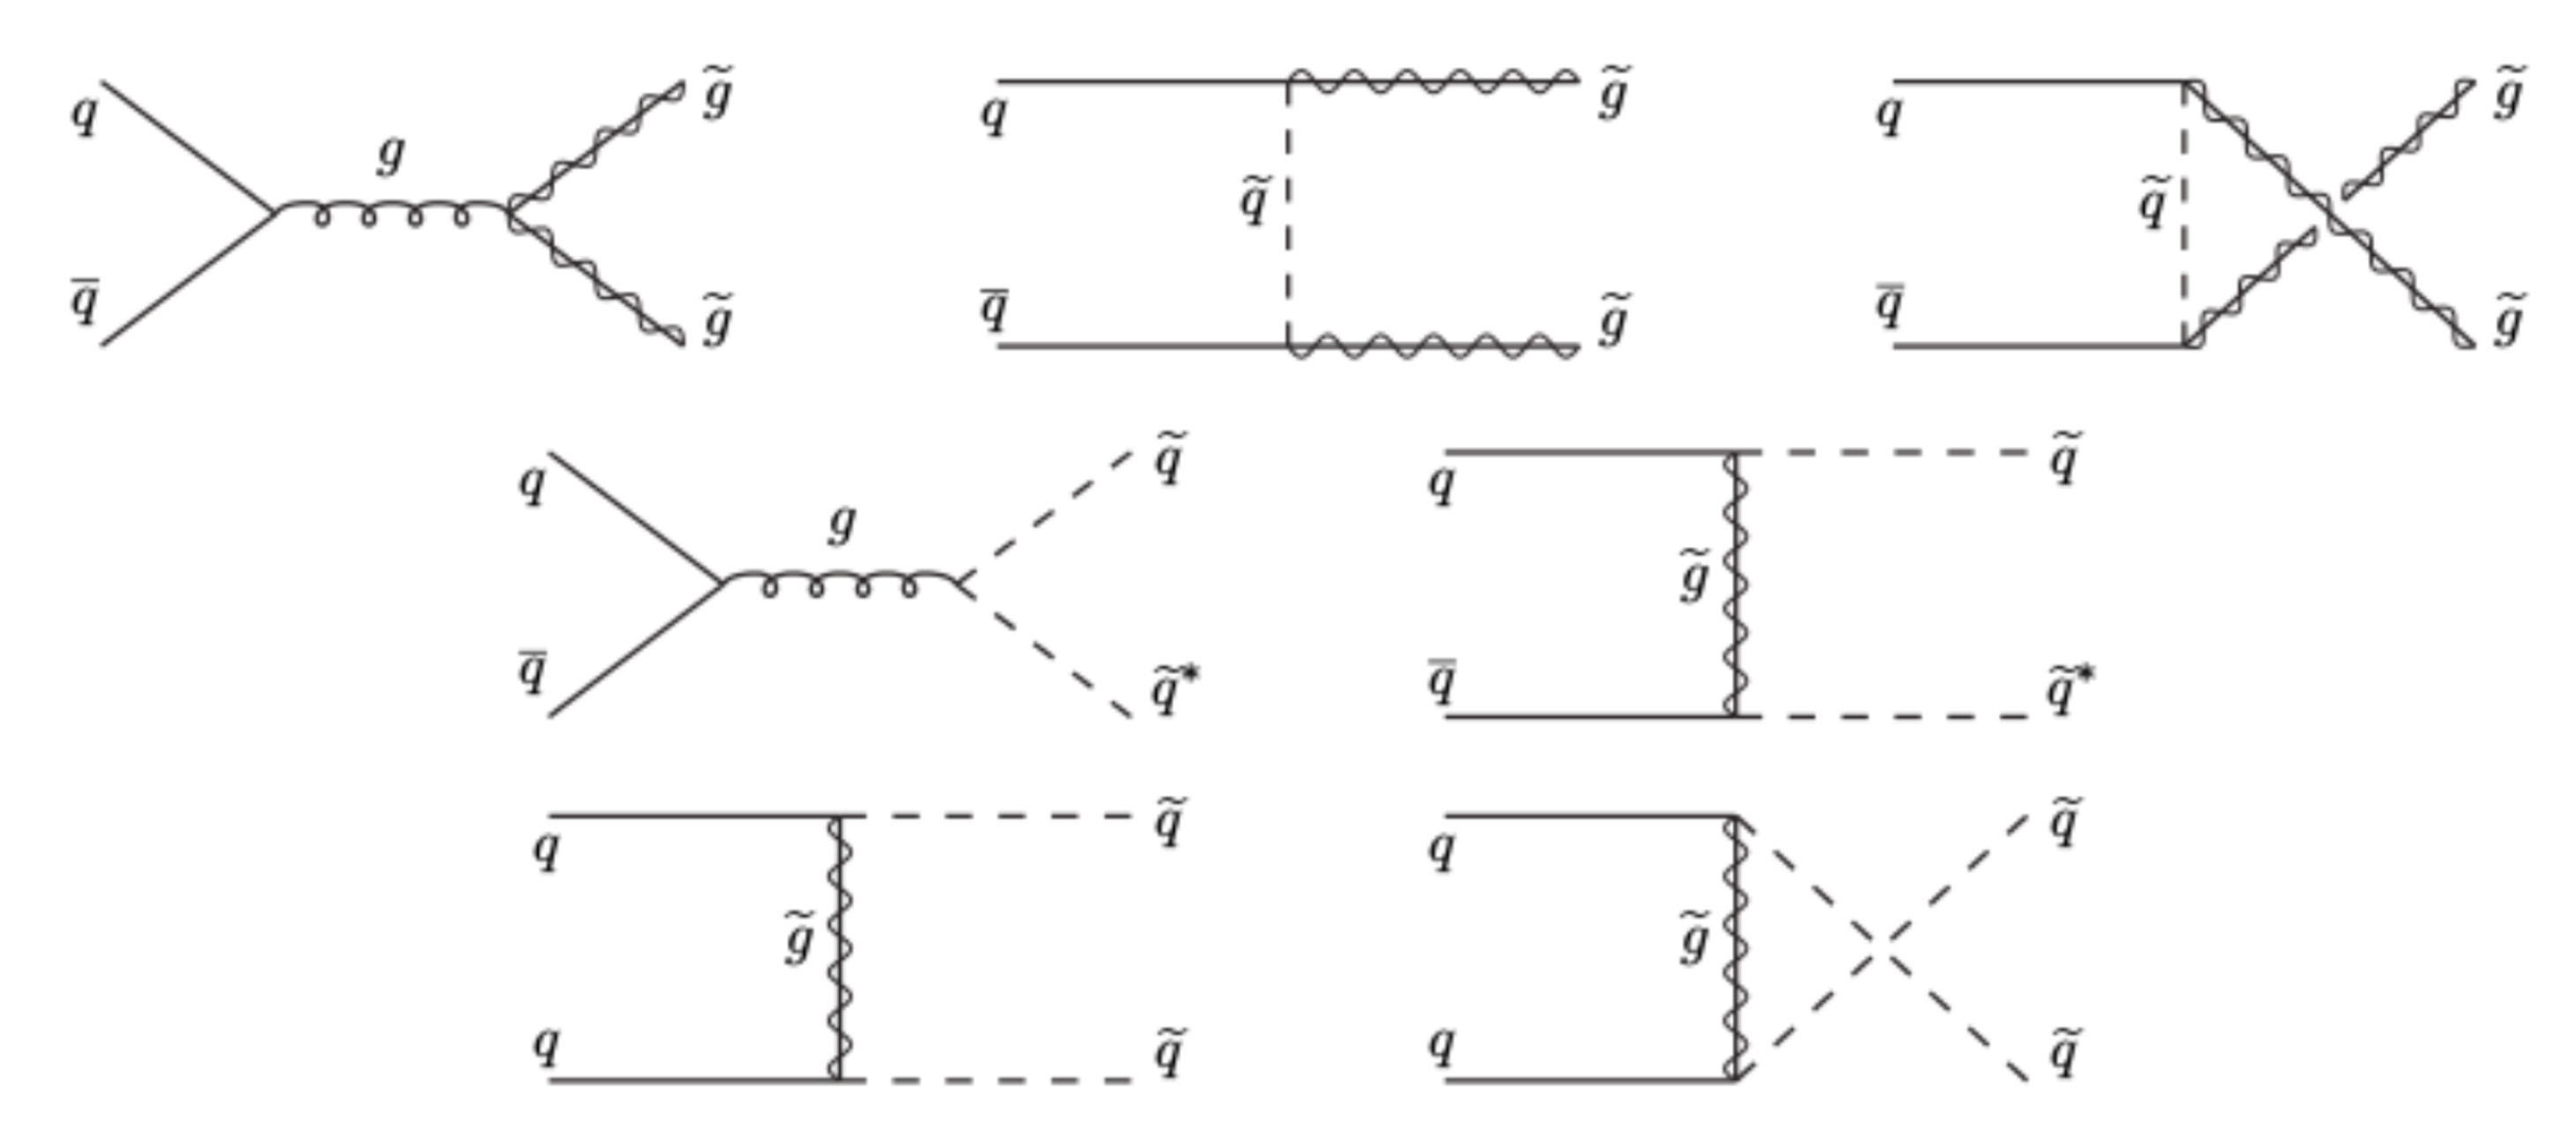
\includegraphics[width=0.6\textwidth]{figures/figure_103}
  \caption{Diagramas de Feynman para la producción de gluinos y squarks en
    colisionadores de hadrones vía aniquilación quark-antiquark y dispersión
    quark-quark}
  \label{fig:strongprod2}
\end{figure}


%% En Tevatron, los procesos de produccion de charginos y neutralinos tienden a tener
%% mayores seccion eficaz, a menos los squarks o el gluino sean muy liviano (menos a 300 \gev,
%% masas que ya se encuentran excluidas por el LHC). En el LHC, la situacion es opuesta, con la
%% produccion de gluinos y squarks dominante por medio de gluon-gluon y gluon-quark fusion.
%% En ambos colisionadores, puede haber produccion asociada de chargino o neutralino junto con
%% un squark y un gluino, pero la mayoria de los modelos predicen que la seccion eficaz
